%
%  THESISBOEK
%
%  Dit bestand zorgt voor algemene (layout)definities, en groepeert de
%  afzonderlijke LaTeX-files tot een geheel.
%
%  @author Erwin Six, David De Reu, Brecht Vermeulen
%

\documentclass[11pt,a4paper,oneside,notitlepage]{book}
\usepackage[english]{babel}
\usepackage{algorithmic}
\usepackage{algorithm}
\usepackage{amsthm}
\usepackage{hyperref}
\usepackage{array}
%\usepackage[nottoc]{tocbibind} % Bibliografie in ToC; zie tocbibind.dvi

% marges aanpassen
% (opmerking: moet *voor* inclusie van fancyhdr package komen)
\setlength{\hoffset}{-1in}
\setlength{\voffset}{-1in}
\setlength{\topmargin}{2cm}
\setlength{\headheight}{0.5cm}
\setlength{\headsep}{1cm}
\setlength{\oddsidemargin}{3.5cm}
\setlength{\evensidemargin}{3.5cm}
\setlength{\textwidth}{16cm}
\setlength{\textheight}{23.3cm}
\setlength{\footskip}{1.5cm}

\usepackage{fancyhdr}
\usepackage{graphicx}
% \usepackage[colorlinks]{hyperref}
% Het bibliografisch opmaak bestand.
\bibliographystyle{unsrt}
%\bibliographystyle{bibliodutch}
%\bibpunct{[}{]}{,}{n}{,}{,}

\newtheorem{mydef}{Definition}

\pagestyle{fancy}

\renewcommand{\chaptermark}[1]{\markright{\MakeUppercase{#1}}}
\renewcommand{\sectionmark}[1]{\markright{\thesection~#1}}

\newcommand{\headerfmt}[1]{\textsl{\textsf{#1}}}
\newcommand{\headerfmtpage}[1]{\textsf{#1}}

\fancyhf{}
\fancyhead[LE,RO]{\headerfmtpage{\thepage}}
\fancyhead[LO]{\headerfmt{\rightmark}}
\fancyhead[RE]{\headerfmt{\leftmark}}
\renewcommand{\headrulewidth}{0.5pt}
\renewcommand{\footrulewidth}{0pt}

\fancypagestyle{plain}{ % eerste bladzijde van een hoofdstuk
  \fancyhf{}
  \fancyhead[LE,RO]{\headerfmtpage{\thepage}}
  \fancyhead[LO]{\headerfmt{\rightmark}}
  \fancyhead[RE]{\headerfmt{\leftmark}}
  \renewcommand{\headrulewidth}{0.5pt}
  \renewcommand{\footrulewidth}{0pt}
}

% anderhalve interlinie (opm: titelblad gaat uit van 1.5)
\renewcommand{\baselinestretch}{1.5}

% indien LaTeX niet goed splitst, neem je woord hierin op, of evt om splitsen 
% te voorkomen
\hyphenation{ditmagnooitgesplitstworden dit-woord-splitst-hier}

\begin{document}

% titelblad (voor kaft)
%  Titelblad

% Opmerking: gaat uit van een \baselinestretch waarde van 1.5 (die moet
% ingesteld worden voor het begin van de document environment)

\begin{titlepage}

\setlength{\hoffset}{-1in}
\setlength{\voffset}{-1in}
\setlength{\topmargin}{1.5cm}
\setlength{\headheight}{0.5cm}
\setlength{\headsep}{1cm}
\setlength{\oddsidemargin}{3cm}
\setlength{\evensidemargin}{3cm}
\setlength{\footskip}{1.5cm}
\enlargethispage{1cm}
% \textwidth en \textheight hier aanpassen blijkt niet te werken

\fontsize{12pt}{14pt}
\selectfont

\begin{center}


\includegraphics[height=2cm]{fig/ruglogo}

\vspace{0.5cm}

Faculteit Toegepaste Wetenschappen\\
Vakgroep Informatietechnologie\\
Voorzitter: Prof.~Dr.~Ir.~Dani\"{e}l~de~Zutter

\vspace{3.5cm}

\fontseries{bx}
\fontsize{17.28pt}{21pt}
\selectfont

Identifying experts through a framework for\\
knowledge extraction from public online source

\fontseries{m}
\fontsize{12pt}{14pt}
\selectfont

\vspace{.6cm}

by 

\vspace{.4cm}

Simon Buelens, Mattias Putman

\vspace{3.5cm}

Promotors: Prof.~Dr.~Ir.~Filip~De~Turck,~Elena~Tsiporkova~(Sirris)\\
Scriptiebegeleiders: Anna~Hristoskova,~Tom~Tourw\'{e}~(Sirris)\\

\vspace{2cm}

Masterproef ingediend tot het behalen van de academische graad van\\
Master in de ingenieurswetenschappen: computerwetenschappen

\vspace{1cm}

Academiejaar 2010--2011

\end{center}
\end{titlepage}


% lege pagina (!!)

% titelblad (!!)

% geen paginanummering tot we aan de inhoudsopgave komen
\pagestyle{empty}

% voorwoord met dankwoord en toelating tot bruikleen (ondertekend)
%%  Voorwoord (dankwoord) en toelating tot bruikleen

\newpage

\noindent \textbf{\huge Dankwoord}

\vspace{1.5cm}

\noindent
We willen vooreerst de gelegenheid aangrijpen om een aantal mensen te bedanken. 
\\

\noindent
We danken onze begeleiders Elena Tsiporkova, Tom Tourw\'e, Anna Hristoskova en Tim Wauters voor de goeie inzichten, de aangename vergaderingen en hun eeuwige geduld.
\\

\noindent
Daarnaast willen we Anne-Sophie Delbecque immens veel bedanken voor het annoteren van de testset, een tijdrovend en eentonig werk.
\\

\noindent
Tot slot bedanken we ook onze families voor de goede zorgen en het vele geduld gedurende de volledige studies in het algemeen en deze moeilijke periode in het bijzonder.

\vspace{1.5cm}

\noindent

\addvspace{4cm}

\noindent Simon Buelens en Mattias Putman, augustus 2011\newpage

\noindent \textbf{\huge Toelating tot bruikleen}

\vspace{1.5cm}

\noindent
``De auteur geeft de toelating deze scriptie voor consultatie beschikbaar
te stellen en delen van de scriptie te kopi\"eren voor persoonlijk
gebruik.\\
Elk ander gebruik valt onder de beperkingen van het auteursrecht,
in het bijzonder met betrekking tot de verplichting de bron uitdrukkelijk
te vermelden bij het aanhalen van resultaten uit deze scriptie.''

\addvspace{4cm}

\noindent Simon Buelens en Mattias Putman, augustus 2011\newpage


%!!!!!!!!!!!!!!!!!!!!!!!!!!!!!!!!!!!!!!!!!!!!!!!!!!!!!!!!!!!!!!!!!!!!!!!!!!!!!!!!!!!!!!!!!!!!!!!!!
%!!!!!!!!!!!              onderaan/bovenaan elk blad thesistitel zetten                !!!!!!!!!!!
%!!!!!!!!!!!!!!!!!!!!!!!!!!!!!!!!!!!!!!!!!!!!!!!!!!!!!!!!!!!!!!!!!!!!!!!!!!!!!!!!!!!!!!!!!!!!!!!!!

% overzicht/samenvatting
%%  Overzichtsbladzijde met samenvatting

\newpage

{
\setlength{\baselineskip}{32pt}
\setlength{\parindent}{0pt}
\setlength{\parskip}{18pt}

\begin{center}

\noindent \textbf{\huge
Identifying experts through }
\textbf{\huge a framework for knowledge extraction}
\textbf{\huge from public online sources}

\setlength{\baselineskip}{12pt}
\setlength{\parindent}{0pt}
\setlength{\parskip}{12pt}

door 

Simon Buelens, Mattias Putman

Promotors: Prof.~Dr.~Ir.~Filip~De~Turck,~Elena~Tsiporkova~(Sirris),~Tom~Tourw\'{e}~(Sirris)\\
Scriptiebegeleiders: Anna~Hristoskova,~Tim~Wauters\\

Masterproef ingediend tot het behalen van de academische graad van\\
Master in de ingenieurswetenschappen: computerwetenschappen

Academiejaar 2010-2011\\
Faculteit Ingenieurswetenschappen\\
Voorzitter: Prof. Dr. Ir. Dani\"{e}l De Zutter\\
Vakgroep Informatietechnologie\\

\end{center}

\setlength{\baselineskip}{10pt}
\setlength{\parindent}{0pt}
\setlength{\parskip}{10pt}

\renewcommand{\baselinestretch}{1.1} 	% De interlinie afstand wat vergroten.
\small\normalsize                       % Nodig om de baselinestretch goed te krijgen.

\section*{Samenvatting}

Onderzoekers verliezen veel tijd met de zoektocht naar informatie gerelateerd aan hun onderzoeksdomein. Er bestaan bijna geen diensten die toelaten om aan de hand van trefwoorden een overzicht te verkrijgen met experts voor de opgegeven domeinen. Er is onderzoek naar disambiguatie van auteurs, maar deze worden meestal niet in combinatie gebracht met het opzoeken van experten, maar het indelen van publicaties (alhoewel de twee gerelateerd zijn).

In deze masterproef onderzoeken we de mogelijkheid om een framework op te stellen dat dit toelaat door online informatie op te zoeken, deze informatie in relatie te brengen met de correcte auteurs en gebruikers toe te laten dit framework te gebruiken om hierin te zoeken. De nadruk van het framework ligt op de disambiguatie van auteurs (aan de hand van de aanwezige informatie alle namen zo goed mogelijk connecteren met de juist auteur) aan de hand van een regelgebaseerde aanpak en de uitbreidbaarheid van het framework.

We maken gebruik van een graafgebaseerde representatie van de data en de architectuur is gebaseerd op pipes en filters. Dit laat toe dat het framework uitbreidbaar, schaalbaar en eenvoudig aanpasbaar is. Op het einde volgen de resultaten gebaseerd op een manueel geannoteerde testset. Uiteindelijk gaan we ook de vergelijking aan met de verdeling van auteurs door DBLP.

\section*{Trefwoorden}

auteur disambiguatie, data verwerking, clustering, pipes en filters

}

\newpage % strikt noodzakelijk om een header op deze blz. te vermijden


\pagestyle{fancy}
\frontmatter

% inhoudstafel
\tableofcontents

% opmaak voor het eigenlijke boek; onderstaande lijnen
% weglaten als de eerste regel van een nieuwe alinea moet
% inspringen in plaats van extra tussenruimte
\setlength{\parindent}{0pt}
\setlength{\parskip}{0.5\baselineskip plus 0.5ex minus 0.2ex}
\setlength{\parskip}{1ex plus 0.5ex minus 0.2ex}

% hoofdstukken
\mainmatter

% hier worden de hoofdstukken ingevoegd (\includes)
\chapter{Introduction}

Researchers are spending a lot of their total research and development hours searching for information. If we could speed up the process of finding the correct information, researchers would have more time to spend on their research and development, the main point of focus.

Leading search engines mainly provide keyword-based results in response of a search query. This is both limited in terms of accuracy and efficiency of information comprehension. Researchers still have to bend over backwards in order to find more information about authors, their level of expertise and their connections. A new type of information service is required which focuses on this problem. It should search the desired information and connect, combine and analyze it in the greater picture of the semantic available information on the internet in order to provide as much value to the user as possible.

% Doelstelling

\section{Thesis objective and approach}

We want to help in this upcoming research by creating a framework that can retrieve experts for any given subject matter. The end result should allow anyone to query the framework with a set of keywords defining the subject area they want to investigate. The outcome of this query is a list of authors, ranked by decreasing level of expertise defined by the dictated keywords. Each author is accompanied by a profile, containing a list of papers, highly touted co-authors and any other information the user might find useful.

We split the internal functioning of this framework in three main components: retrieving information from various online sources (publications, author profiles or online presentations), analyzing this information and linking it to a specific author (a proces we call clustering) and defining the areas of interest of each author and their level of expertise for each of these areas.

For the first component, we limited ourselves to using DBLP \cite{dblp} as online source. This is a service providing bibliographic information on major computer science journals and proceedings. We limit ourselves to this one source as the information is comparable to other listings, while they provide an XML overview for each publication allowing us to parse it with ease. It is still sufficiently challenging, as publications are often attributed to the wrong author. We considered adding author profiles from LinkedIn, but this often complicated it as profiles were often inaccessible, incomplete or outdated.

In the second component, each publication we retrieve from DBLP is saved as a unique instance and each author is initially considered different from any previous ones. Clustering consists of linking authornames to distinct authors. This is the key component for this thesis and is what we focused on the most. We have composed various rules based on name similarity, recurring co-authors, publication subjects, affiliation and email address. These rules are used by the framework to calculate similarities between publications and authors. As more information is obtained, the framework dynamically updates the clusters containing publications from the same author.

The last component is responsible for defining the area of interest of an author. In order to accomplish this, a category tree is created. Each publication is then mapped onto this tree and the combination of all the publications form a subtree which is linked an author's interests. To decide the level of expertise, the number of subject references, the number of publication citations and the level of expertise of co-authors should be combined. However, this is beyond the scope of our thesis and we have simplified this by comparing the subject of the publications extracted from the title and the abstract and the number of publications for each subject.

%To tackly this problem, we split it in two main parts. The first consists of retrieving and analyzing information about authors from various online sources. This includes defining what publications map to what authors, a proces we call clustering and which is the key component of this thesis, and retrieving the subjects of each publication. 
%
%The proces of clustering is the main point of interest of this thesis. Linking publications to authors is a lot harder than just comparing names. Authors may have the exact same name, names can be misspelled and names can be shortened or altered. In \autoref{} we define a set of rules combining attributes of authors and relationships between them. In \autoref{} we test combinations of these rules to find the best outcome.
%
\section{Chapter outline}

The first chapter is this introduction and describes the objective of our thesis and how we want to accomplish this.

In \autoref{sota}, we start with a summary of existing technologies and techniques that we researched. Afterwards, we describe the different thesis topics we examined. For each topic, we discuss the existing research and 

% TODO bespreek onze werkmethode op een zodanige manier dat een 'expert' (bv. medestudent) door de beschrijving verstaat waarom we deze bepaalde aanpak gekozen hebben

% TODO bespreek hoe de hoofdstukken in elkaar zitten (overzicht)

\chapter{State of the art}

We examined a broad range of different topics with social media as central subject. It was an evolution starting from simple Twitter-related subjects to a full-fledged problem assignment many people struggle with. 
%The journey towards this problem is interesting enough to devote a full thesis to in itself, but we will spare you the details and cover it in this chapter.

\section{Opinion mining}

\subsection{Introduction}
\label{general - opinion mining}
Opinion mining is part of the general area of \textit{sentiment analysis, opinion extraction or opinion mining and feature-based opinion summarization} from the user-generated content or user-generated media on the Web. The applications are manifold with the most important ones in the area of in business intelligence. 

%Large companies receive thousands of pieces of feedback on a daily basis, both direct as indirect. Examples are online customer reviews, customer feedback, survey responses, social media messages, blogposts and comments. Human processing of such text volumes is prohibitively expensive and close to impossible. The only alternative is automatic extraction of relevant information. Ideally one would like to be able to quickly and cheaply customize a system to provide reasonably accurate sentiment classification for a domain, a brand or a specific product.

\subsection{Current situation}

%Sentiment360, lots of papers and onderzoek, really to much to name and to add something of importance.

Opinion mining has been a hot topic the last 10 years due to the rise of social media such as blogs and social networks. Businesses are looking to automate the process of following up on the conversation about their company image and products and opinion mining can help them take steps toward accomplishing this \footnote{Wright, Alex. "Mining the Web for Feelings, Not Facts", New York Times, 2009-08-23. Retrieved on 2010-11-05}.

One step towards this is accomplished in research. Several universities around the world have research teams focussing on the dynamics of sentiment. There is research focused on creating sentiment summaries to capture an author's opinion about a subject based on a publication \footnote{An exploration of sentiment summarization}, predicting the semantic orientation of adjectectives and combinations of adjectives \footnote{Predicting the Semantic Orientation of Adjectives}, identifying the sources of the opinions rather than the actual sentiment itself \footnote{Identifying Sources of Opinions with Conditional Random Fields and Extraction Patterns}...

An interesting ongoing project is \footnote{http://www.cs.uic.edu/~liub/FBS/sentiment-analysis.html} at the University of Illinois, Chicago, backed by Google and Microsoft Corporation. It is a project working in three areas: 

\begin{itemize}
	\item Mining direct (or regular) opinions. Example: after taking the drug, I got stomach pain.
	\item Mining comparative opinions. Example: Coke tastes better than Pepsi.
	\item Review and opinion spam analysis and detection. An example is detecting of fake reviews.
\end{itemize}

It is particularly interesting as others can follow the status of and updates on the project. There are also references to the opinion lexicon and data sets they used to evaluate their results allowing third parties to easily compare their own work using the same input.

\subsection{Improvements and additions}

%Voorloping nog heel erg dunnetjes, Google Prediction API is het enige dat we aanbrengen en dit is meer iets simpel uitvoeren dan echt een uitdagende opdracht. Beter de uitdaging van Twitter aankaarten en hoe we dit concreet wouden aanpakken.

We are looking into the analysis of social media messages, more specifically Twitter messages. We want to use Google's new service, Google Prediction API, which provides pattern-matching and machine learning capabilities. We can compare the results with one or more of the many papers and see if there is any added value in using this service.

We need a lot of training data in order for the Prediction API to learn likely future outcomes. As this service decides what algorithms it uses, there is a lack of possible research to make an interesting thesis.


%Zeer veel onderzoek en bestaande tools, mogelijke uitbreidingen zijn beperkt en toepassingen ook.

%\subsection{Bijlage}
%http://code.google.com/intl/nl-NL/apis/predict/

\section{Twitter influencers}

\subsection{Introduction}
As discussed in \ref{general - opinion mining} about opinion mining, people talk about products, both positive as negative. They have the ability to influence the buying behavior of others who respect their opinion about a certain area. Identifying these influencers can be of great value, for instance in the advertising industry.

There are two main aspects, reach and trust. A person's reach determines the number of people who listen when he has something of value to say. Trust or influence depicts the value people give a certain person's opinion. Both aspects can vary a lot when comparing different topics for the same person.

\subsection{Current situation}

There are papers discussing algorithms to find the ideal subset of individuals which will trigger a large cascade of conversions and papers researching the more general economic issues regarding influencers.

Also regarding the second aspect, trust, there are a lot of well documented scientific results. \footnote{Propagation Models for Trust and Distrust in Social Networks} describes propagation models which can be used to present trust and distrust in social networks. Just as in \footnote{Inferring Trust Relationships in Web-based Social Networks} an algorithm for calculating a trust metric is presented based on the EigenTrust algorithm\footnote{The eigentrust algorithm for reputation management in p2p networks, Kamvar 2003}.

The amount of applications focusing on calculating social media influence, as their core business or a useful option, is growing rapidly. Following is a short summary a few better applications.

Klout is a well-known online tool focusing on ranking Twitter profiles (and recently also Facebook profiles) using over 35 variables. These rankings are, though fun, not particularly useful as finding influencers based on topic is very limited, however there are interesting third-party applications providing this feature.

PeerIndex and Traackr focus more on identifying topics. Just like Klout, PeerIndex focuses on Twitter profiles and parameters captured from Twitter to assign a certain score to each profile. Traackr on the other hand uses data from multiple online sources connected to the users such as their blog, YouTube channel, LinkedIn and Twitter profile and more. Traackr combines the results and provides a three-way score (reach, relevance and resonance) based on a certain topic together with detailed contact information.

\subsection{Improvements and additions}

%We kunnen hier nog zo veel meer over vertellen, dit is eigelijk de voornaamste voorloper van ons echt onderwerp, dus hier kunnen we reeds heel wat belangrijke dingen aankaarten die we uiteindelijk ook echt zullen gebruiken. 
%Belangrijke dingen die nog aangekaart moeten worden: Semantic Web (Web of Data), DBPedia, RDF, OWL, FOAF, Google Social Graph, location based?, 

We want to start from a Twitter profile and find out more about a user using other social media networks, semantic databases and social graphs, comparable to Traackr. 

%\section{Event detection}
%
%\subsection{General problem statement}
%
%
%\subsection{Current situation}
%
%\subsection{Improvements and additions}


\section{Expert Finding}

\subsection{Introduction}

Finding experts is useful for seeking consultants, collaborators or speakers. It is also of great value within the academic world as it provides a source of information to supplement or complement papers and theses. Many researchers and reporters lose a lot of time doing this manually as the amount of sources is ever growing: documents, email, databases, conferences, scientific papers and so on. The topic is luckily seeing an increase in attention in recent years.

%Expert finding is a difficult task requiring a multitude of different steps in order to find results bearing certain value. There are databases containing records of people matched with their area of expertise, which can be queried for a nominal fee, mostly used by reporters. The data has been gathered manually over time. To receive a more up-to-date or specific result, one will have to send a separate request which will come with a higher price and take its time.\\
%Another option is to do it manually. There are several steps which can be undertaken and they can be executed in fashionable order, repeated as often as necessary. One can search for conference sites about the topic and look up the names of the speakers. Current and past working experience can possibly be found on LinkedIn. Publications and co-authors can be retrieved from online databases with dedicated research publications or from more general databases such as Google Scholar. The authors and papers can be interlinked in order to see who works with who and who is most often cited or referenced. Influence can be measured on social media.\\
%It is clearly a lengthy process.

\subsection{Current situation}

\footnote{Balog, K. and Rijke, M.: Finding Experts and Their Details in E-mail Corpora. In Proceedings
of the 15th International Conference on World Wide Web (2006)} proposed four simple binary association methods to find expertise information from emails. \footnote{5} investigated the expertise of users and experts by combining information retrieval techniques. Both these solutions are insufficient for topic-based expert finding as their datasets (emails and online communities) are too limited, they focus too much on previous encounters and lack context.

\footnote{6} retrieves experts based on the amount of documents persons have for a given topic. As input a keyword phrase is used in order to find relevant documents. The results are however unsatisfactory caused by its slow response time and incorrect relationship between persons and documents. \footnote{8} gets better results using an algorithm based on a PageRank for document authority, a co-occurrence model for authors and multiple levels of associations between experts and topics. It succeeds to map variants of experts' names on the same author, but fails to identify different authors with the same name.

\footnote{Finding Topic-centric Identified Experts based on Full Text Analysis} proposes OntoFrame. It is an information service platforum using Semantic Web technologies and is based on an extensive ontology of 16 classes using RDF triples. Identity resolution and full text analysis forms the basis of their expert-finding method. The framework looks promising, however the prototype does not function \footnote{$http://ontoframe.kr/2008/2008_new/main.jsp$}.

\subsection{Improvements and additions}

%Iets vermelden over de connectie met het TWIRL project?

We want to continue the research proposed in \footnote{Finding Topic-centric ...}, but less focused towards the full text analysis of documents. We want to create a platform that extracts and unifies the required information from a variety of online sources and subsequently builds a repository of user profiles.

%Te bespreken: neo4j, Tinkerpop, Gremlin, Stanford POS tagger, lemmatizer, doc split (ruby gem), resque (ruby library - https://github.com/defunkt/resque), max flow :: min-cut

%\subsection{What do we need}

%%%%%%%%%%%%%%%%%%%%%%%%%%%%%%%%%%%%%%%%%%%%%%%%%%%%%%%%%%

%% Several components we still have to explain or discuss inside the text %%

\subsection{Web scraping}

Web scraping (also called Web harvesting or Web data extraction) is a computer software technique of extracting information from websites. Usually, such software programs simulate human exploration of the Web by implementing low-level Hypertext Transfer Protocol (HTTP). Web scraping focuses on the transformation of unstructured data on the Web, typically in HTML format, into structured data that can be stored and analyzed in a central local database or spreadsheet. Web scraping is also related to Web automation, which simulates human Web browsing using computer software \footnote{http://en.wikipedia.org/wiki/Web scraping}.

We will use scraping in several of our plugins to collect information about authors and publications as we don't have a large database with this information and constructing one ourselves would take too much time and resources. The downside is that it is typically a slow process as the content of each page has to be downloaded and parsed by the computer.

\subsection{API}

\subsection{DBLP}

DBLP is produced by the Computer Science department of the University of Trier and was initially focused on \textit{DataBase systems and Logic Programming}, but has gradually expanded toward being an confidential server providing bibliographic information on major computer science journals and proceedings, indexing more than one million articles.
DBLP allows to search by author name, giving back a list of publications and other bibliographic information.

DBLP does not provide us with an API, so we will use web scraping in order to extract all the necessairy information.

%Link naar de volledige uitleg van de werking van de plugin voor meer informatie hieromtrent

\subsection{LinkedIn}

LinkedIn is a business-related social networking site launched in May 2003, mainly used for professional networking by more than 100 million registered users \footnote{http://en.wikipedia.org/wiki/LinkedIn}. Each user has a profile which may contain the following information: current affiliation and title, past working experiences, education, specialties, location, connections with other users...

Using the LinkedIn API we can search for users by entering a name. This will give back list of profiles we can browse and whose information we can extract and use in our framework. As the service is based on a \textit{gated-access approach}, which means you need to be at least a second level connection of the profile you are looking at to see their connections, we can not use this to connect authors to eachother. However, the information provided by the profile which is publicly available does allow us to get a better insight into the subject the person is interested in and what affiliation he is and was connected to.

%Link naar de volledige uitleg van de werking van de plugin voor meer informatie hieromtrent

\subsection{Google Scholar}

Google Scholar is a freely accessible web search engine that indexes the full text of scholarly literature accross an array of publishing formats and disciplines. It allows to search publications based on subject keywords, partial publication titles and author names. It's ranking algorithm uses a combination of factors, but puts mainly high weight to citation count and the words included in a document's title.

Google Scholar is not yet available to the Google AJAX API and Google does not allow automatic crawling or scraping of its services. Thus, it can not be used as a publication reference in our framework.

\subsection{Microsoft Academic Search}

Microsoft Academic Search is a free search engine for academic papers and resources principally in the field of computer science, developed by Microsoft Research Asia, Beijing. The database consists of the bibliographic information (metadata) for academic papers published in journals, conferences proceedings and the citations between them. Objects are ranked according to two factors: their relevance to the query, which is computed by its attributes; and their global importance, calculated by its relationships with other objects \footnote{http://en.wikipedia.org/wiki/Microsoft Academic Search}.

It is a direct competitor of Google Scholar and it allows us to scrape the information of the site, making it useful to extract publications written by a specific author, his fields of interest, the amount of times he was cited and his co-authors for our framework.

\subsection{FOAF}

FOAF is a descriptive vocabulary expressed using the Resource Description Framework (RDF) and the Web Ontology Language (OWL). Computers may use these FOAF profiles to find, for example, all people living in Europe, or to list all people both you and a friend of yours know. This is accomplished by defining relationships between people. Each profile has a unique identifier (such as the person's e-mail addresses, a Jabber ID, or a URI of the homepage or weblog of the person), which is used when defining these relationships \footnote{http://en.wikipedia.org/wiki/FOAF (software)}.

% Meer uitleggen wat wij hier mee zijn en hoe dit gebruikt kan worden.

\subsection{Stemming}

\subsection{Clustering}

\subsection{Stanford Part-Of-Speech Tagger}

%http://nlp.stanford.edu/software/tagger.shtml

A Part-Of-Speech Tagger, or POS Tagger, is a piece of software that reads text in some language and assigns parts of speech to each word (and other token), such as noun, verb, adjective, etc., although generally computational applications use more fine-grained POS tags like 'noun-plural'. The Stanford POS Tagger is Java implementation of the log-linear part-of-speech taggers described in the papers \footnote{Kristina Toutanova and Christopher D. Manning. 2000. Enriching the Knowledge Sources Used in a Maximum Entropy Part-of-Speech Tagger. In Proceedings of the Joint SIGDAT Conference on Empirical Methods in Natural Language Processing and Very Large Corpora (EMNLP/VLC-2000), pp. 63-70.} and \footnote{Kristina Toutanova, Dan Klein, Christopher Manning, and Yoram Singer. 2003. Feature-Rich Part-of-Speech Tagging with a Cyclic Dependency Network. In Proceedings of HLT-NAACL 2003, pp. 252-259.}.

We will use this POS Tagger to determine the nouns and adjectives in the publication title which, on their turn, will be used to determine the subject of the publication as 

\subsection{Gremlin}

\subsection{JUNG}

\subsection{Neo4j}

\chapter{The framework}

\section{Main Scenario}

The goal is to build a platform that allows a user to query for experts in a particular domain. The
platform extracts and unifies the required information from a variety of online sources and
subsequently builds a repository of user profiles. We basically want to create a framework that would function as a Google for finding experts given a certain subject.

We will use the following steps to build such a platform:

%verduidelijken dat de volgorde van deze stappen niet belangrijk is, ze zijn interchangeable

\begin{itemize}
	%Welke auteur namen ? Waar halen we die vandaan ? Conference sites ?
	\item \textbf{Seed data} We need a list of author names to start with.
	\item \textbf{Information extraction}
		\begin{itemize}
			\item Looking up personal information, ie. profiles from LinkedIn.
			\item Looking up publications, extracting title, co-authors and affiliation. The co-authors can be used as new input for further information extraction.
			\item Categorize publications by subject
		\end{itemize}
	\item \textbf{Disambiguation} Decide if there are different authors with the same name or different spellings of the same author's name which should be mapped to one author.
\end{itemize}

A simplified representation of these steps can be seen on \ref{fig:db-gegevens}. It shows the steps that are responsible for finding the data that we will store in our database and which will be used to find experts.

\begin{figure}[htbp]
	\centering
		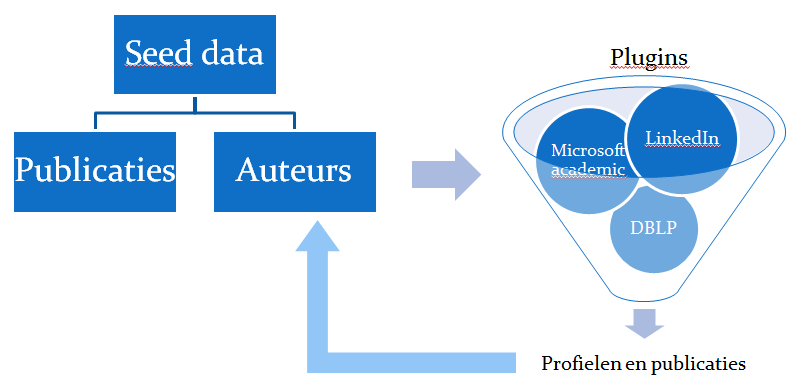
\includegraphics[width=0.75\textwidth]{fig/database-gegevens.png}
	\caption{A simplified representation of the different steps our framework takes to find data about experts.}
	\label{fig:db-gegevens}
\end{figure}

%Describe how we got to the architecture for the framework, show a figure of the (simplified + extensive) architecture and explain the different components.

\section{Features}

Based on the main scenario, we can identify a few key features our framework will need. A short summarization of each follows, explaining the challenges we face with our thesis. Each of these features will be discussed more deeply throughout this chapter.

%Beter verwijzen waar ze meer informatie per feature kunnen doornemen?

\subsection{Information extraction}

We need to extract information from multiple sources, which we will accomplish by using a plugin system. Each plugin is responsible for one source and will extract specific information which can be used by other plugins or other steps in our framework.

\subsection{Categorization}

In order to decide who is an expert regarding a certain subject, we will have to decide the subject of expertise of each author. A very important part of this will be in deciding the subject of the publications. The challenge is to decide this using as few information as possible, preferably by just inspecting the title, as getting access to the text of the publication itself is a whole lot more time- and resource-consuming.

\ref{categorybuilder} describes this more in-depth.

\subsection{Disambiguation}

A challenging feature is the disambiguation. There are two reasons. The first is the fact that an author's name is not a unique reference for a person. There might be multiple authors with the same name, which means we have to take this into account when deciding who is an expert. Secondly, a name might be spelled differently or changed throughout time. Examples are abbreviations, an extra family name because of a marriage or simply spelling errors.

More on disambiguation can be found in \ref{disambiguator}, describing the component responsible for the disambiguation.

\subsection{Dynamic}

There is a big dynamic concept tied to our thesis. People who are experts on a certain subject a decade ago, may not be as important anymore now or may have changed their subject of expertise. An interesting point of view would be to enable users to scroll through a timeline so they could see the changes themselves. This is however out of the scope of our thesis.

\section{Architecture}

Based on the scenario, we came up with the necessary components our framework needs. \ref{fig:architectuur} shows a simplistic version of how the architecture will look like. The different components of the framework and their connection toward eachother is displayed. In the next sections, the most important components will be explained at large.

% TODO : say something about the seed data and scoperfu.rb ?

\begin{figure}[htbp]
	\centering
		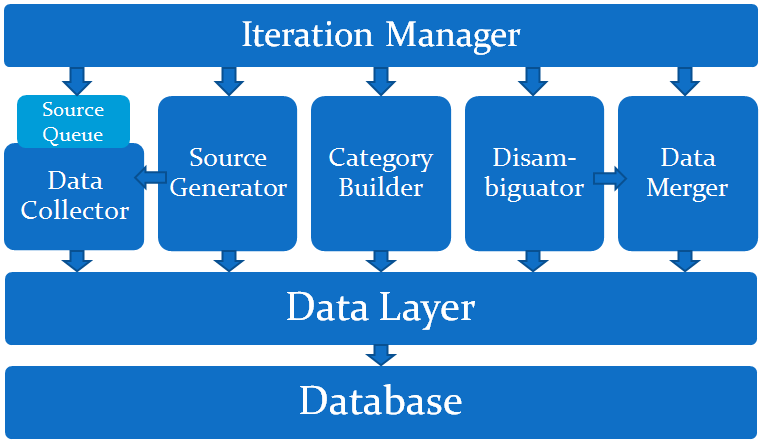
\includegraphics[width=0.75\textwidth]{fig/architectuur.png}
	\caption{First attempt at the architecture based on the necessary components}
	\label{fig:architectuur}
\end{figure}

\subsection{Iteration Manager}

This component is responsible for the flow of the entire framework. It knows what iteration our program is at and knows what the next steps are. It calls the necessary components and hands it the correct parameters in order for it to execute it's code. This will become clearer when we explain the next components.

\subsection{Data Collector}

The Data Collector receives sources from the Source Generator. It will call each of these plugins with the parameters received from the Iteration Manager, updating the database with the new data the plugins generate.

\subsection{Source Generator}

This component holds a collection of plugins, each responsible for generating data to be used by our framework coming from one source, and sends the a reference of the needed, decided by the Iteration Manager, plugins to the Source Queue in the Data Collector. 

There are different kind of plugins, according to the possible data that can be extracted. This data can include background information about a name, like location, affiliation, work experience or university. Other plugins extract information about publications (title, authors, date...) and yet another might be responsible for collecting the pdf of a publication.

%For more information about the different plugins and how they work, please refer to ??
%We want to/have set up our framework to allow new plugins to be made and used easily, extending the possibilities and usages.
% TODO : Delete this next line and either make a reference to a better explanation or better explain it here.

The different plugins we use are based on LinkedIn for personal information and DBLP en Microsoft Academic Search for bibliographic information.

% TODO : reference a plugin which is responsible for finding the pdf (something based on Google Scholar).

\subsection{Category Builder}
\label{categorybuilder}

%Category builder is eigelijk verantwoordelijk voor het opstellen van de categorie boom, zou beter zijn moest dit verantwoordelijk zijn voor het assignen van een category aan een publicatie (of een auteur?) en alles wat hier komt bij te kijken.

The Category Builder's role is deciding the subject(s) of the publications and assigning it to a category which fits in a category tree.

% TODO : Uitleg hoe dit precies in zijn werk gaat, gebruik makende van de Wikipedia API, Stanford POS Tagger.

We have two main possibilties to decide the subject of a publication. The first is by only focusing on the publication title, the second is by also making use of the actual text in the publication. The second will yield us with better results, but getting the text and analysing it will take a lot more time than just analysing a few words. 

For both manners in deciding the subject, we will make use of the Stanford Part-of-speech Tagger. We use it to select the adjectives and nouns, as these contain the most interesting information regarding to deciding the field of the publication.

When only having the publication title, the words marked by the Stanford POS Tagger will be searched on Wikipedia, by use of the API. We will search for the words seperately and make combinations, based on the closeness of the words in their original context.

% TODO : more information of HOW exactly this will work? What happens after we search them on Wikipedia ? How do we decide which ones are crap, which ones aren't ? Probably better to dedicate a whole section for the Category Builder.

When we have the original text of the publication, the easiest method is scanning for the keywords. These are often cited after the abstract and give us a very quick enumeration of the subjects discussed in the article. Another possibility is parsing the abstract itself by using the same algorithm explained above, used on the publication title.


\subsection{Disambiguator}
\label{disambiguator}

The disambiguation is an important factor towards the strength of our framework. In the data collection phase, we view each name as e new object in our database, even if that name is already stored. This is necessairy to keep the option open that the same name might be connected towards different authors. This also means our database grows fast. 

The disambiguation exists out of a number of rules. These inspect several objects in the database and define the probabilities that names, typically connected to a publication or a profile, are connected to eachother and to one author. %These probabilities are stored as weights of edges between these objects.

An in-depth explanation of these rules can be found in \ref{disamb_rules}.

\subsection{Data Merger}

The Data Merger is responsible for merging the names together so they would reference to the same author. This component uses the probabilities calculated by the Disambiguator in order to do so.

%\section{Technologies}
%
%\subsection{MySQL}
%
%Discuss the differences, advantages and disadvantages between a relational datastore, a record-store and a triple-store.
%
%\subsubsection{Relational datastore}
%
%\subsubsection{A record-store}
%
%\subsubsection{Triple-store}
%
%\subsubsection{Conclusion}
%
%We choose to use MySQL, a relational datastore, because we are familiar with it. It allows us to quickly set up our prototype to work and test our framework on.
%
%\subsection{Two databases}
%
%We use two databases, one for development and one for production.
%
%The former is used to collect all information about the possible experts and their work. 
%
%\subsection{Ruby}

\section{Disambiguation rules}

Every publication will have a number of authors tied to it and each author is in first instance saved as a seperate identity. However, as we expand our database a lot of names will relate to the same author. In order to find these relationships, it is not enough to just compare the notation using string-matching. Different authors may have the same name and an author's name may be misspelled or abbreviated.

In order to map the names onto an identity, we came up with a number of rules. Each of these increase or decrease the likelihood that two names should map to the same author. We use this likelihood to decide if names should be tied to the same author or disconnected, a dynamic process as we collect more and more information.

%Per regel zouden we een soort van gewicht moeten meegeven die genormaliseerd is over alle regels heen. Hier moeten we nog over nadenken.
%Misschien moeten we ook per regel verwijzen naar een plaats in het boek waar dit beter uitgelegd wordt, bv Interest rule in combinatie met Category builder.

\subsection{Prequel - Doc split}

In order to enlarge our disambiguation possibilities, we want access to the actual text of the publications. Using a search engine, like Google Scholar, we can find most of the actual publications in pdf on the internet. By using the Ruby library Doc split \footnote{http://documentcloud.github.com/docsplit/}, we can easily parse the pdf into computer-understandable text. Most of the time it will be enough to just get the first page, giving us access to the authors, their affiliations and location. The first page also almost always has an abstract and a list of keywords.

%Nog nodig van dit duidelijker aan te duiden. Sommige regels kunnen opgesplitst worden in 2 versies, versie met en zonder. Dus misschien eerst opsomming van regels die er geen gebruik van maken, daarna opsomming van regels die dit wel doen.
In the following rules we will make a distinction between those who rely on this extra information and those who don't. The rule who rely on it will be followed by an asterisk *.

\subsection{Place of publication rule*}

This rule defines that is less likely to have multiple persons with the exact same name writing a publication in the same city.

\subsection{Co-author clustering}

%Slecht uitgelegd, gebruik maken van een figuur ?

Authors often work together with the same people, writing multiple publications together. If we find clusters 
%\footnote{how do we formally define clusters and where do we explain this concept? Should this be in the sota related towards the publication 'Clustering using min cut tree'?} 
of co-authors which are completely indepent, it enlarges the probability that name we are investigating is related to multiple authors.

We can also use this rule to enlarge the possibility of author names being related by using this rule the other way around. When we have a big cluster of related co-authors, the change is big the author correlated to this cluster is the same person.

\subsection{Name notation rule}

Using string matching to detect similarities between names which are written differently, but are the same person. Examples include abbreviations of firstnames, usage of special characters, double family names...

\subsection{Affiliation rule*}

It is unlikely for an author to be tied towards multiple affiliations at the same time.

\subsection{Interest rule}

This is an important rule and it can define a lot of the precision of our whole framework. It states that different authors with the same name are unlikely to work on the same topic or have the same area of expertise.

The hard part is deciding the subject of the publication.

\chapter{Important components}

\section{Disambiguator}

\section{Disambiguation rules}

Every publication will have a number of authors tied to it and each author is in first instance saved as a seperate identity. However, as we expand our database a lot of names will relate to the same author. In order to find these relationships, it is not enough to just compare the notation using string-matching. Different authors may have the same name and an author's name may be misspelled or abbreviated.

In order to map the names onto an identity, we came up with a number of rules. Each of these increase or decrease the likelihood that two names should map to the same author. We use this likelihood to decide if names should be tied to the same author or disconnected, a dynamic process as we collect more and more information.

%Per regel zouden we een soort van gewicht moeten meegeven die genormaliseerd is over alle regels heen. Hier moeten we nog over nadenken.
%Misschien moeten we ook per regel verwijzen naar een plaats in het boek waar dit beter uitgelegd wordt, bv Interest rule in combinatie met Category builder.

\subsection{Prequel - Doc split}

In order to enlarge our disambiguation possibilities, we want access to the actual text of the publications. Using a search engine, like Google Scholar, we can find most of the actual publications in pdf on the internet. By using the Ruby library Doc split \footnote{http://documentcloud.github.com/docsplit/}, we can easily parse the pdf into computer-understandable text. Most of the time it will be enough to just get the first page, giving us access to the authors, their affiliations and location. The first page also almost always has an abstract and a list of keywords.

%Nog nodig van dit duidelijker aan te duiden. Sommige regels kunnen opgesplitst worden in 2 versies, versie met en zonder. Dus misschien eerst opsomming van regels die er geen gebruik van maken, daarna opsomming van regels die dit wel doen.
In the following rules we will make a distinction between those who rely on this extra information and those who don't. The rule who rely on it will be followed by an asterisk *.

\subsection{Place of publication rule*}

This rule defines that is less likely to have multiple persons with the exact same name writing a publication in the same city.

\subsection{Co-author clustering}

%Slecht uitgelegd, gebruik maken van een figuur ?

Authors often work together with the same people, writing multiple publications together. If we find clusters 
%\footnote{how do we formally define clusters and where do we explain this concept? Should this be in the sota related towards the publication 'Clustering using min cut tree'?} 
of co-authors which are completely indepent, it enlarges the probability that name we are investigating is related to multiple authors.

We can also use this rule to enlarge the possibility of author names being related by using this rule the other way around. When we have a big cluster of related co-authors, the change is big the author correlated to this cluster is the same person.

\subsection{Name notation rule}

Using string matching to detect similarities between names which are written differently, but are the same person. Examples include abbreviations of firstnames, usage of special characters, double family names...

\subsection{Affiliation rule*}

It is unlikely for an author to be tied towards multiple affiliations at the same time.

\subsection{Interest rule}

This is an important rule and it can define a lot of the precision of our whole framework. It states that different authors with the same name are unlikely to work on the same topic or have the same area of expertise.

The hard part is deciding the subject of the publication.

\section{Clustering algorithm}

\subsection{Introduction}

The core of our framework is the algorithm responsible for deciding what nodes match to the same author, based on similarities between these nodes. These similarities are the output generated by the rules implemented in the Disambiguator. Using these similarities the algorithm can create new information which could be new input for the Disambiguator. It is clear that we need a dynamic approach as there is a constant flow of new information.

We need an efficient algorithm for clustering and it has to be able to handle a steady stream of new information while maintaining an optimal solution. These clusters contain instances which map to the same author and will be used to determine the field of expertise for each author later on. The quality of this algorithm will make or break the quality of the output of our framework.

For the algorithm we based ourselves largely on the algorithm described in \cite{saha2006dynamic}. An efficient dynamic algorithm is described for clustering graphs for handling insertion and deletion of edges, maintaining high quality clusters as defined by the quality requirement given in \cite{flake2004graph}. The algorithm makes heavy use of the minimum-cut tree. We implemented Gusfield's algorithm, based on \cite{rodrigues2011mpi}, and will explain this first.

The main feature of this dynamic algorithm is that it only builds part of the minimum-cut tree as and when necessary. The tree is computed over a subset of nodes, limited to a number of clusters. In our graph there might be an immense number of authors, and thus clusters. However, the amount of authors involved with one change is limited. By just computing the clusters of this coarsened graph we can obtain the clusters of the original graph. These two properties are the reason the algorithm is efficient while maintaining an identical cluster quality as the static version described in \ref{staticcutclustering}. Formal proof for this quality can be found in \cite{saha2006dynamic}.

\subsection{Minimum-cut tree algorithm}
\label{minimumcuttree}

\begin{algorithm}
\caption{Sequential Gusfield's Algorithm}
\label{mincutgusfield}
\begin{algorithmic}
\STATE \textbf{Input:} $G = (V,E,w)$ 
\STATE \textbf{Output:} $T = (V,E,f)$, where T is a cut tree of G
\STATE $V(T) \leftarrow V(G); E(T) \leftarrow \emptyset$
\FOR{$tree_i, flow_i, 1 \leq i \leq N$}
\STATE $tree_i \leftarrow 1; flow_i \leftarrow 0$
\ENDFOR
\STATE // $n - 1$ maximum flow iterations
\FOR{$s \leftarrow 2 $to$ N$}
\STATE $flow_s \leftarrow $MaxFlow$(s, tree_s)$
\STATE // adjust the $tree$ with Cut($s,tree_s$)
\STATE // c1 contains s and connected nodes, c2 contains $tree_s$ and connected nodes
	\FOR{$t \leftarrow 1 $ to $ N$}
		\IF{$t == s \vee t == tree_s$}
			\STATE next
		\ELSIF{$t \in c1 \wedge s \in c2$}
			\STATE $tree_t \leftarrow s$
		\ELSIF{$t \in c2 \wedge s \in c1$}
			\STATE $tree_t \leftarrow tree_s$
		\ENDIF
	\ENDFOR
\ENDFOR
\STATE // Generate T
\FOR{$s \leftarrow 1 $ to $ N$}
\STATE $E(T) \leftarrow E(T) \cup {s, tree_s}$
\STATE $f({s,tree_s}) \leftarrow flow_s$
\ENDFOR
\RETURN T
\end{algorithmic}
\end{algorithm}

% Perhaps this first paragraph should be moved to the SOTA

We briefly explain what is understood under a minimum cut tree, as clarified in \cite{saha2006dynamic}. 

Let $G = (V,E,w)$ denote a weighted undirected graph with $n = |V|$ nodes or vertices and $m = |E|$ links or edges. Each edge $e = (u, v), u,v \in V$ has an associated weight $w(u,v) > 0$. Let $s$ and $t$ be two nodes in $G(V,E)$, the source and destination. The minimum-cut of G with respect to $s$ and $t$ is a partition of $V$ which we will call $S$ and $V/S$. These partitions should be such that $s \in S, t \in V/S$ and the total weight of the edges linking nodes between the two partitions is minimum. The sum of these weights is called the cut-value and is denoted as $c(S,V/S)$. 

The minimum cut tree is a tree on $V$ such that inspecting the path between $s$ and $t$ in the tree, the minimum-cut of $G$ with respect of $s$ and $t$ can be obtained. Removal of the minimum weight edge in the path yields the two partitions and the weight of the corresponding edge gives the cut-value.

We implemented a sequential version of Gusfield's algorithm which calculates the minimum cut tree of any given graph. The pseudocode is given by \ref{mincutgusfield}. In the pseudocode we use numbers to point to nodes or vertices. These numbers can be choosen randomly.

The algorithm consists of $n-1$ iterations of a Maximum Flow algorithm and for every iteration a different vertex is chosen as source. The destination vertex is determined by previous iterations and is saved in the tree. Initially all vertices of the output tree point to node 1, but this can be adjusted after each iteration. This adjustment depends on the minimum-cut between the current source and destination. We split all the nodes in two collections, using this minimum-cut. We adjust the parent of each node if it is on another side as its current parent, which is stored in the tree.

We choose an implementation of the Edmonds-Karp algorithm to find the maximum flow and the minimum-cut. This algorithm is an implementation of the Ford-Fulkerson method for computing the maximum flow and is provided to us through the java library JUNG.

\subsection{Cut clustering}

\cite{flake2004graph} defines a static algorithm for clustering based on minimum cut trees. \ref{staticcutclustering} gives the pseudocode of the basic cut clustering algorithm. It adds an artificial sink $t$ to all the vertices of the graph with weight $\alpha > 0$. The minimum cut tree is computed using this new graph and the disjoint components obtained after removing the artificial vertex $t$, are the required clusters.

\begin{algorithm}
\caption{Static Cut Clustering Algorithm of \cite{flake2004graph}}
\label{staticcutclustering}
\begin{algorithmic}
\STATE \textbf{Input:} $G = (V,E,c), \alpha$ 
\STATE \textbf{Output:} Cluster of G
\STATE $V \leftarrow V \cup t$
\FOR{all vertices $v$ in G}
	\STATE Connect $t$ to $v$ with edge of weight $\alpha$
\ENDFOR
\STATE $G'(V',E') \leftarrow$ new graph after connecting t to V
\STATE Calculate the minimum-cut tree $T'$ of $G'$
\STATE Remove $t$ from T
\RETURN All connected components as clusters of G
\end{algorithmic}
\end{algorithm}

In \cite{saha2006dynamic}, they have extended this basic algorithm allowing it to work efficiently on dynamic graphs. They use some important new components which we also will use throughout the explanation of the algorithm. The adjacency matrix $A$ of $G$ is an $n \times n$ matrix in which $A(i,j) = w(i,j)$ if $(i,j) \in E$, else $A(i,j) = 0$. The algorithm also maintains two new variables for every vertex, the In Cluster Weight (ICW) and the Out Cluster Weigh (OCW). If $C_1,C_2,...C_s$ are the clusters of $G(V,E)$ then ICW and OCW are defined as below.

\begin{mydef}
\textbf{In Cluster Weight (ICW)} of a vertex $v \in V$ is defined as the total weight of the edges linking the vertex $v$ to all the vertices which belong to the same cluster as $v$. That is, if $v \in C_i$, $0 \leq i \leq s$ then $ICW(v) = \sum_{u \in C_i}{w(v,u)}$
\end{mydef}

\begin{mydef}
\textbf{Out Cluster Weight (OCW)} of a vertex $v \in V$ is defined as the total weight of the edges linking the vertex $v$ to all the vertices which do not belong to the same cluster as $v$. That is, if $v \in C_i$, $0 \leq i \leq s$ then $OCW(v) = \sum_{u \in C_j, j \neq i}{w(v,u)}$
\end{mydef}

Receiving new information is represented as a new edge between two nodes with a given weight. The weight represents the amount the two nodes are connected, this is calculated by the rules in the disambiguator. There are two different possibilities that have to be treated separatly, named inter- and intra-cluster edge addition.

We assume we have $C = {C_1,C_2...C_s}$ as the clusters of the graph $G(V,E)$ which have been calculated in previous steps. We denote $A$ as the adjacency matrix of $G$.

\paragraph{Intra-cluster edge addition}

Intra-cluster edge addition means that both the nodes of the added edge belong to the same cluster. The result is that the cluster becomes better connected. We only have to update the $ICW$ and the adjacency matrix $A$ while the nodes remain unchanged. \ref{intracluster} shows the pseudocode.

\begin{algorithm}
\caption{Intra-cluster edge addition between nodes $i$ and $j$ with weight $w(i,j)$}
\label{intracluster}
\begin{algorithmic}
\STATE \textbf{Input:} $G(V,E), (i,j), w(i,j)$ 
\STATE \textbf{Output:} Clusters of G
\STATE $A(i,j) \leftarrow A(i,j) + w(i,j)$
\STATE $ICW(i) \leftarrow ICW(i) + w(i,j)$
\STATE $ICW(j) \leftarrow ICW(j) + w(i,j)$
\RETURN $C$
\end{algorithmic}
\end{algorithm}

\paragraph{Inter-cluster edge addition}

Addition of an edge whose end nodes belong to different clusters is more challenging as it increases the connectivity across different clusters. This means the cluster quality of the clusters involved is lowered and as a result reclustering might be necessary when the cluster quality is no longer maintained. 

There are three identifiable cases:

\begin{enumerate}
	\item \textbf{CASE 1} The addition of the edge does not break the clusters involved
	\item \textbf{CASE 2} The addition of the edge causes the clusters to be so well connected that they are merged into one
	\item \textbf{CASE 3} The new edge deteriorates the cluster quality and the nodes in both the clusters have to be reclustered
\end{enumerate}

In order to understand the complete algorithm shown in \ref{intercluster} for inter-cluster edge addition which also uses the minimum-cut tree algorithm discussed in \ref{minimumcuttree}, we have to explain two new processes: merging and contraction of clusters.

\subparagraph{Merging of clusters} occurs in CASE 2 and is described in \ref{merging}. Two clusters $C_u$ and $C_v$ are merged into one new cluster containing the nodes of the two original clusters. This causes the ICW of all the nodes involved to increase and the OCW to decrease as all the nodes are now more connected.

\begin{algorithm}
\caption{Merging of clusters $C_u$ and $C_v$}
\label{merging}
\begin{algorithmic}
\STATE \textbf{Input:} $C_u$ and $C_v$ 
\STATE \textbf{Output:} Merged cluster
\STATE $D \leftarrow C_u \cup C_v$
\FOR{$\forall u \in C_u$}
	\STATE $ICW(u) \leftarrow ICW(u) + \sum_{v \in C_v}{w(u,v)}$
	\STATE $OCW(u) \leftarrow OCW(u) - \sum_{v \in C_v}{w(u,v)}$
\ENDFOR
\FOR{$\forall v \in C_v$}
	\STATE $ICW(v) \leftarrow ICW(v) + \sum_{u \in C_u}{w(v,u)}$
	\STATE $OCW(v) \leftarrow OCW(v) - \sum_{u \in C_u}{w(v,u)}$
\ENDFOR
\RETURN $D$
\end{algorithmic}
\end{algorithm}

\subparagraph{Contraction of clusters} occurs in CASE 3 as part of the reclustering process and is shown in \ref{contracting}. All the nodes outside the set of clusters $S$ are replaced by a single new node $x$. Self loops that are created in this process are removed and parallel edges are replaced by a single edge with weight equal to the sum of the parallel edges. The reason we consider the clusters outside $S$ is because $S$ will generally be small while the other clusters will contain a lot of nodes.

\begin{algorithm}
\caption{Contraction of clusters outside the set of clusters $S$}
\label{contracting}
\begin{algorithmic}
\STATE \textbf{Input:} $G(V,E)$ and set of clusters $S$ 
\STATE \textbf{Output:} Contracted graph $G'(V',E')$
\STATE Add all vertices of $S$ to a new graph $G'$
\STATE $\forall i,j \in V' : A'(i,j) \leftarrow A(i,j)$
\STATE Add a new vertex $x$ to $G'$
\FOR{$\forall i \in \left\{V' - x\right\}$}
	\STATE $A'(i,x) = ICW(i) + OCW(i) - \sum_{j \in \left\{ V' - x \right\} }{A'(i,j)}$
\ENDFOR
\STATE Obtain $E'$ from $A'$
\RETURN $G'(V',E')$
\end{algorithmic}
\end{algorithm}


\begin{algorithm}
\caption{Inter-cluster edge addition between nodes $i$ and $j$ with weight $w(i,j)$}
\label{intercluster}
\begin{algorithmic}
\STATE \textbf{Input:} $G(V,E), (i,j), w(i,j)$ and $\alpha$ 
\STATE \textbf{Output:} Clusters of $G$
\STATE $i \in C_u$ and $j \in C_v$
\IF{$\frac{\sum_{u \in C_u}{OCW(u) + w(i,j)}}{\left|V - C_u\right|} \leq \alpha \wedge \frac{\sum_{v \in C_v}{OCW(v) + w(i,j)}}{\left|V - C_v\right|} \leq \alpha$}
	\STATE // CASE 1
	\STATE $A(i,j) \leftarrow A(i,j) + w(i,j)$
	\STATE $OCW(i) \leftarrow OCW(i) + w(i,j)$
	\STATE $OCW(j) \leftarrow OCW(j) + w(i,j)$
	\RETURN $C$
\ELSIF{$\frac{2 * c(C_u,C_v)}{V} \geq \alpha$}
	\STATE // CASE 2
	\STATE $D \leftarrow MERGE(C_u,C_v)$
	\RETURN $C + D - \left\{C_u,C_v\right\}$
\ELSE
	\STATE // CASE 3
	\STATE $G'(V',E') \leftarrow CONTRACT(G(V,E),\left\{C_u,C_v\right\} )$
	\STATE Connect $t$ to $v, \forall v \in C_u,C_v$ with edge of weight $\alpha$
	\STATE Connect $t$ to $V' - \left\{C_u, C_v\right\}$ with edge of weight $\alpha * \left\| V - C_u - C_v \right\|$
	\STATE G''(V'',E'') is the graph resulting in connecting $t$
	\STATE Calculate minimum-cut tree $T''$ of $G''(V'',E'')$
	\STATE Remove $t$
	\STATE // $\left\{D_1,D_2...D_k\right\}, k > 0$, are the connected components of $T''$ after removing $t$
	\STATE $C \leftarrow \left\{D_1,D_2...D_k,C_1,C_2...C_s\right\} - \left\{ C_u,C_v \right\}$
	\RETURN $C$
\ENDIF
\end{algorithmic}
\end{algorithm}

% TODO : bij merge, moet A, OCW en ICW updaten en bij CASE 3 hetzelfde, dit wordt niet vermeld in de paper en ook nog niet in onze pseudocode

\section{Clustering algorithm}

\subsection{Introduction}

The core of our framework is the algorithm responsible for deciding what nodes match to the same author, based on similarities between these nodes. These similarities are the output generated by the rules implemented in the Disambiguator. Using these similarities the algorithm can create new information which could be new input for the Disambiguator. It is clear that we need a dynamic approach as there is a constant flow of new information.

We need an efficient algorithm for clustering and it has to be able to handle a steady stream of new information while maintaining an optimal solution. These clusters contain instances which map to the same author and will be used to determine the field of expertise for each author later on. The quality of this algorithm will make or break the quality of the output of our framework.

For the algorithm we based ourselves largely on the algorithm described in \cite{saha2006dynamic}. An efficient dynamic algorithm is described for clustering graphs for handling insertion and deletion of edges, maintaining high quality clusters as defined by the quality requirement given in \cite{flake2004graph}. The algorithm makes heavy use of the minimum-cut tree. We implemented Gusfield's algorithm, based on \cite{rodrigues2011mpi}, and will explain this first.

The main feature of this dynamic algorithm is that it only builds part of the minimum-cut tree as and when necessary. The tree is computed over a subset of nodes, limited to a number of clusters. In our graph there might be an immense number of authors, and thus clusters. However, the amount of authors involved with one change is limited. By just computing the clusters of this coarsened graph we can obtain the clusters of the original graph. These two properties are the reason the algorithm is efficient while maintaining an identical cluster quality as the static version described in \ref{staticcutclustering}. Formal proof for this quality can be found in \cite{saha2006dynamic}.

\subsection{Minimum-cut tree algorithm}
\label{minimumcuttree}

\begin{algorithm}
\caption{Sequential Gusfield's Algorithm}
\label{mincutgusfield}
\begin{algorithmic}
\STATE \textbf{Input:} $G = (V,E,w)$ 
\STATE \textbf{Output:} $T = (V,E,f)$, where T is a cut tree of G
\STATE $V(T) \leftarrow V(G); E(T) \leftarrow \emptyset$
\FOR{$tree_i, flow_i, 1 \leq i \leq N$}
\STATE $tree_i \leftarrow 1; flow_i \leftarrow 0$
\ENDFOR
\STATE // $n - 1$ maximum flow iterations
\FOR{$s \leftarrow 2 $to$ N$}
\STATE $flow_s \leftarrow $MaxFlow$(s, tree_s)$
\STATE // adjust the $tree$ with Cut($s,tree_s$)
\STATE // c1 contains s and connected nodes, c2 contains $tree_s$ and connected nodes
	\FOR{$t \leftarrow 1 $ to $ N$}
		\IF{$t == s \vee t == tree_s$}
			\STATE next
		\ELSIF{$t \in c1 \wedge s \in c2$}
			\STATE $tree_t \leftarrow s$
		\ELSIF{$t \in c2 \wedge s \in c1$}
			\STATE $tree_t \leftarrow tree_s$
		\ENDIF
	\ENDFOR
\ENDFOR
\STATE // Generate T
\FOR{$s \leftarrow 1 $ to $ N$}
\STATE $E(T) \leftarrow E(T) \cup {s, tree_s}$
\STATE $f({s,tree_s}) \leftarrow flow_s$
\ENDFOR
\RETURN T
\end{algorithmic}
\end{algorithm}

% Perhaps this first paragraph should be moved to the SOTA

We briefly explain what is understood under a minimum cut tree, as clarified in \cite{saha2006dynamic}. 

Let $G = (V,E,w)$ denote a weighted undirected graph with $n = |V|$ nodes or vertices and $m = |E|$ links or edges. Each edge $e = (u, v), u,v \in V$ has an associated weight $w(u,v) > 0$. Let $s$ and $t$ be two nodes in $G(V,E)$, the source and destination. The minimum-cut of G with respect to $s$ and $t$ is a partition of $V$ which we will call $S$ and $V/S$. These partitions should be such that $s \in S, t \in V/S$ and the total weight of the edges linking nodes between the two partitions is minimum. The sum of these weights is called the cut-value and is denoted as $c(S,V/S)$. 

The minimum cut tree is a tree on $V$ such that inspecting the path between $s$ and $t$ in the tree, the minimum-cut of $G$ with respect of $s$ and $t$ can be obtained. Removal of the minimum weight edge in the path yields the two partitions and the weight of the corresponding edge gives the cut-value.

We implemented a sequential version of Gusfield's algorithm which calculates the minimum cut tree of any given graph. The pseudocode is given by \ref{mincutgusfield}. In the pseudocode we use numbers to point to nodes or vertices. These numbers can be choosen randomly.

The algorithm consists of $n-1$ iterations of a Maximum Flow algorithm and for every iteration a different vertex is chosen as source. The destination vertex is determined by previous iterations and is saved in the tree. Initially all vertices of the output tree point to node 1, but this can be adjusted after each iteration. This adjustment depends on the minimum-cut between the current source and destination. We split all the nodes in two collections, using this minimum-cut. We adjust the parent of each node if it is on another side as its current parent, which is stored in the tree.

We choose an implementation of the Edmonds-Karp algorithm to find the maximum flow and the minimum-cut. This algorithm is an implementation of the Ford-Fulkerson method for computing the maximum flow and is provided to us through the java library JUNG.

\subsection{Cut clustering}

\cite{flake2004graph} defines a static algorithm for clustering based on minimum cut trees. \ref{staticcutclustering} gives the pseudocode of the basic cut clustering algorithm. It adds an artificial sink $t$ to all the vertices of the graph with weight $\alpha > 0$. The minimum cut tree is computed using this new graph and the disjoint components obtained after removing the artificial vertex $t$, are the required clusters.

\begin{algorithm}
\caption{Static Cut Clustering Algorithm of \cite{flake2004graph}}
\label{staticcutclustering}
\begin{algorithmic}
\STATE \textbf{Input:} $G = (V,E,c), \alpha$ 
\STATE \textbf{Output:} Cluster of G
\STATE $V \leftarrow V \cup t$
\FOR{all vertices $v$ in G}
	\STATE Connect $t$ to $v$ with edge of weight $\alpha$
\ENDFOR
\STATE $G'(V',E') \leftarrow$ new graph after connecting t to V
\STATE Calculate the minimum-cut tree $T'$ of $G'$
\STATE Remove $t$ from T
\RETURN All connected components as clusters of G
\end{algorithmic}
\end{algorithm}

In \cite{saha2006dynamic}, they have extended this basic algorithm allowing it to work efficiently on dynamic graphs. They use some important new components which we also will use throughout the explanation of the algorithm. The adjacency matrix $A$ of $G$ is an $n \times n$ matrix in which $A(i,j) = w(i,j)$ if $(i,j) \in E$, else $A(i,j) = 0$. The algorithm also maintains two new variables for every vertex, the In Cluster Weight (ICW) and the Out Cluster Weigh (OCW). If $C_1,C_2,...C_s$ are the clusters of $G(V,E)$ then ICW and OCW are defined as below.

\begin{mydef}
\textbf{In Cluster Weight (ICW)} of a vertex $v \in V$ is defined as the total weight of the edges linking the vertex $v$ to all the vertices which belong to the same cluster as $v$. That is, if $v \in C_i$, $0 \leq i \leq s$ then $ICW(v) = \sum_{u \in C_i}{w(v,u)}$
\end{mydef}

\begin{mydef}
\textbf{Out Cluster Weight (OCW)} of a vertex $v \in V$ is defined as the total weight of the edges linking the vertex $v$ to all the vertices which do not belong to the same cluster as $v$. That is, if $v \in C_i$, $0 \leq i \leq s$ then $OCW(v) = \sum_{u \in C_j, j \neq i}{w(v,u)}$
\end{mydef}

Receiving new information is represented as a new edge between two nodes with a given weight. The weight represents the amount the two nodes are connected, this is calculated by the rules in the disambiguator. There are two different possibilities that have to be treated separatly, named inter- and intra-cluster edge addition.

We assume we have $C = {C_1,C_2...C_s}$ as the clusters of the graph $G(V,E)$ which have been calculated in previous steps. We denote $A$ as the adjacency matrix of $G$.

\paragraph{Intra-cluster edge addition}

Intra-cluster edge addition means that both the nodes of the added edge belong to the same cluster. The result is that the cluster becomes better connected. We only have to update the $ICW$ and the adjacency matrix $A$ while the nodes remain unchanged. \ref{intracluster} shows the pseudocode.

\begin{algorithm}
\caption{Intra-cluster edge addition between nodes $i$ and $j$ with weight $w(i,j)$}
\label{intracluster}
\begin{algorithmic}
\STATE \textbf{Input:} $G(V,E), (i,j), w(i,j)$ 
\STATE \textbf{Output:} Clusters of G
\STATE $A(i,j) \leftarrow A(i,j) + w(i,j)$
\STATE $ICW(i) \leftarrow ICW(i) + w(i,j)$
\STATE $ICW(j) \leftarrow ICW(j) + w(i,j)$
\RETURN $C$
\end{algorithmic}
\end{algorithm}

\paragraph{Inter-cluster edge addition}

Addition of an edge whose end nodes belong to different clusters is more challenging as it increases the connectivity across different clusters. This means the cluster quality of the clusters involved is lowered and as a result reclustering might be necessary when the cluster quality is no longer maintained. 

There are three identifiable cases:

\begin{enumerate}
	\item \textbf{CASE 1} The addition of the edge does not break the clusters involved
	\item \textbf{CASE 2} The addition of the edge causes the clusters to be so well connected that they are merged into one
	\item \textbf{CASE 3} The new edge deteriorates the cluster quality and the nodes in both the clusters have to be reclustered
\end{enumerate}

In order to understand the complete algorithm shown in \ref{intercluster} for inter-cluster edge addition which also uses the minimum-cut tree algorithm discussed in \ref{minimumcuttree}, we have to explain two new processes: merging and contraction of clusters.

\subparagraph{Merging of clusters} occurs in CASE 2 and is described in \ref{merging}. Two clusters $C_u$ and $C_v$ are merged into one new cluster containing the nodes of the two original clusters. This causes the ICW of all the nodes involved to increase and the OCW to decrease as all the nodes are now more connected.

\begin{algorithm}
\caption{Merging of clusters $C_u$ and $C_v$}
\label{merging}
\begin{algorithmic}
\STATE \textbf{Input:} $C_u$ and $C_v$ 
\STATE \textbf{Output:} Merged cluster
\STATE $D \leftarrow C_u \cup C_v$
\FOR{$\forall u \in C_u$}
	\STATE $ICW(u) \leftarrow ICW(u) + \sum_{v \in C_v}{w(u,v)}$
	\STATE $OCW(u) \leftarrow OCW(u) - \sum_{v \in C_v}{w(u,v)}$
\ENDFOR
\FOR{$\forall v \in C_v$}
	\STATE $ICW(v) \leftarrow ICW(v) + \sum_{u \in C_u}{w(v,u)}$
	\STATE $OCW(v) \leftarrow OCW(v) - \sum_{u \in C_u}{w(v,u)}$
\ENDFOR
\RETURN $D$
\end{algorithmic}
\end{algorithm}

\subparagraph{Contraction of clusters} occurs in CASE 3 as part of the reclustering process and is shown in \ref{contracting}. All the nodes outside the set of clusters $S$ are replaced by a single new node $x$. Self loops that are created in this process are removed and parallel edges are replaced by a single edge with weight equal to the sum of the parallel edges. The reason we consider the clusters outside $S$ is because $S$ will generally be small while the other clusters will contain a lot of nodes.

\begin{algorithm}
\caption{Contraction of clusters outside the set of clusters $S$}
\label{contracting}
\begin{algorithmic}
\STATE \textbf{Input:} $G(V,E)$ and set of clusters $S$ 
\STATE \textbf{Output:} Contracted graph $G'(V',E')$
\STATE Add all vertices of $S$ to a new graph $G'$
\STATE $\forall i,j \in V' : A'(i,j) \leftarrow A(i,j)$
\STATE Add a new vertex $x$ to $G'$
\FOR{$\forall i \in \left\{V' - x\right\}$}
	\STATE $A'(i,x) = ICW(i) + OCW(i) - \sum_{j \in \left\{ V' - x \right\} }{A'(i,j)}$
\ENDFOR
\STATE Obtain $E'$ from $A'$
\RETURN $G'(V',E')$
\end{algorithmic}
\end{algorithm}


\begin{algorithm}
\caption{Inter-cluster edge addition between nodes $i$ and $j$ with weight $w(i,j)$}
\label{intercluster}
\begin{algorithmic}
\STATE \textbf{Input:} $G(V,E), (i,j), w(i,j)$ and $\alpha$ 
\STATE \textbf{Output:} Clusters of $G$
\STATE $i \in C_u$ and $j \in C_v$
\IF{$\frac{\sum_{u \in C_u}{OCW(u) + w(i,j)}}{\left|V - C_u\right|} \leq \alpha \wedge \frac{\sum_{v \in C_v}{OCW(v) + w(i,j)}}{\left|V - C_v\right|} \leq \alpha$}
	\STATE // CASE 1
	\STATE $A(i,j) \leftarrow A(i,j) + w(i,j)$
	\STATE $OCW(i) \leftarrow OCW(i) + w(i,j)$
	\STATE $OCW(j) \leftarrow OCW(j) + w(i,j)$
	\RETURN $C$
\ELSIF{$\frac{2 * c(C_u,C_v)}{V} \geq \alpha$}
	\STATE // CASE 2
	\STATE $D \leftarrow MERGE(C_u,C_v)$
	\RETURN $C + D - \left\{C_u,C_v\right\}$
\ELSE
	\STATE // CASE 3
	\STATE $G'(V',E') \leftarrow CONTRACT(G(V,E),\left\{C_u,C_v\right\} )$
	\STATE Connect $t$ to $v, \forall v \in C_u,C_v$ with edge of weight $\alpha$
	\STATE Connect $t$ to $V' - \left\{C_u, C_v\right\}$ with edge of weight $\alpha * \left\| V - C_u - C_v \right\|$
	\STATE G''(V'',E'') is the graph resulting in connecting $t$
	\STATE Calculate minimum-cut tree $T''$ of $G''(V'',E'')$
	\STATE Remove $t$
	\STATE // $\left\{D_1,D_2...D_k\right\}, k > 0$, are the connected components of $T''$ after removing $t$
	\STATE $C \leftarrow \left\{D_1,D_2...D_k,C_1,C_2...C_s\right\} - \left\{ C_u,C_v \right\}$
	\RETURN $C$
\ENDIF
\end{algorithmic}
\end{algorithm}

% TODO : bij merge, moet A, OCW en ICW updaten en bij CASE 3 hetzelfde, dit wordt niet vermeld in de paper en ook nog niet in onze pseudocode

\chapter{Framework Evaluation and Results}
\label{results}


We need to evaluate the performance of the framework. We will mainly focus our tests on the clustering of authors and the influence of different combinations of rules and parameters on the results. Proper clustering results in a collection of publications related to one author, allowing to define specialties and the level of expertise. 

In order to accomplish realistic and useful results, it's important the tests resemble realistic use-cases. This means testing against both general and borderline queries. Parameters making it easier in disambiguation are rare and country specific author names, a multitude of publications which are written with the same co-authors or the inclusion of the same email address. A combination of these parameters allows for easier manual checking of results, but is consequently less challenging. 

Borderline cases make more defiant evaluations. Author names containing foreign characters or accents make it easier to be misspelled. In contrast, common last names also make it harder to differentiate between different authors. Examples are Anderson or Smith in United States, Chen or Lee in East Asian countries or Peters in Belgium.

% Wat moeten we bespreken in dit hoofdstuk:

% De testopstelling
	% Hoe zit deze in elkaar
	% Waarom hebben hiervoor gekozen
	% Vergelijking met anderen?
% De bekomen resultaten
% (Vergelijken met andere mensen)

% Moeten we dit doen voor de clustering (dus vooral kijken naar name disambiguation) en de expert finding (hiervoor hebben we voornamelijk de category builder nodig voor goede resultaten)

\section{Evaluation Setup}

\subsection{Comparative Research}

The authors of \cite{han2004two} focus on disambiguating between authors having the same name or names which are very closely related. They use a dataset consisting of nine different names, each having at least 10 different name variations. For each variation they have collected publications from DBLP. An overview of this dataset can be viewed on \autoref{tab:auth-dblp-dataset} together with the results they achieve using different rules for disambiguation. The mean accuracy they accomplish with their best approach is $73.3\%$ with a standard deviation of $5.4\%$.

\begin{table}
	\centering
		\begin{tabular}[ht]{|c||c|c|c|c|c|c|}
			\hline
			\bfseries{Name} & \bfseries{Variations} & \bfseries{Size} & \bfseries{Coauthor} & \bfseries{Paper} & \bfseries{Journal} & \bfseries{Combination} \\
			\hline
			S Lee & 35 & 244 & 61.3\% & 14.3\% & 43.8\% & 65.4\% \\
			\hline
			J Lee & 33 & 172 & 70.9\% & 17.7\% & 39.9\% & 75.9\% \\
			\hline
			J Kim & 25 & 127 & 57.1\% & 18.8\% & 40.2\% & 66.1\% \\
			\hline
			Y Chen & 24 & 108 & 78.5\% & 14.0\% & 26.9\% & 81.7\% \\
			\hline
			S Kim & 20 & 94 & 69.0\% & 13.8\% & 27.6\% & 70.1\% \\
			\hline
			C Lee & 18 & 80 & 72.2\% & 13.9\% & 43.1\% & 75.0\% \\
			\hline
			A Gupta & 16 & 172 & 75.0\% & 25.6\% & 50.6\% & 78.1\% \\
			\hline
			J Chen & 13 & 91 & 66.3\% & 31.3\% & 44.6\% & 72.3\% \\
			\hline
			H Kim & 11 & 63 & 73.7\% & 21.1\% & 43.9\% & 75.4\% \\
			\hline
			\hline
			\bfseries{Mean} & & & 69.3\% & 18.9\% & 40.0\% & \bfseries{73.3\%} \\
			\hline
			\bfseries{StdDev} & & & 6.8\% & 6.1\% & 7.9\% & 5.4\% \\
			\hline
		\end{tabular}
	\caption{The nine DBLP datasets used in \cite{han2004two}. Each row contains the base name, the number of recorded variations and the total amount of examined publications of this name. The last four columns show the accuracy measured using the different rules. The two bottom rows give the mean accuracy for the rules and the standard deviation.}
	\label{tab:auth-dblp-dataset}
\end{table}

It is important to note that the division of the clusters is solely based on the division of the authors in DBLP. As this division on DBLP is often wrong, we find that this makes a poor benchmark. Getting very high accuracy when comparing to DBLP does not mean the result is good. In order to get a proper insight into the disambiguation quality, we would still have to check the results manually. This is the main reason we choose to compose our own dataset.

\subsection{Test Set}
\label{sec:testset}

As stated before, we want to resemble a realistic combination of easier and harder use-cases for our own dataset. As \autoref{tab:testset} shows, we have chosen five base names, each with a number of variations and have manually disambiguated these variations and combined the authors into clusters using the information on DBLP and the actual papers, if they were available. In total our test set contains just over a 1000 publications. An overview of the names that correspond to each of these base names, can be found in \autoref{appendix:dataset}, together with links to DBLP. In order to make it easier, we will use the following definition in the rest of the text:

\begin{mydef}
	\bfseries{Family} With the term family, we refer to one of the five base names.
\end{mydef}

Nevertheless we composed the clusters manually, there are no guarantees that this is completely accurate. Especially for the families "Chen" and "Johnson", there might be small mistakes as the amount of different authors is overwhelming. However, the dataset we composed is a lot more accurate than DBLP. The comparison between the number of authors represented by DBLP and the number of authors we disambiguated, is also shown on \autoref{tab:testset}.

\begin{table}
	\centering
		\begin{tabular}[ht]{|c|c|c|c|}
			\hline
			\bfseries{Name Set} & \bfseries{Authors} & \bfseries{Publications} & \bfseries{DBLP} \\
			\hline
			Turck & 4 & 172 & 4 \\
			\hline
			Chen & 70 & 221 & 1 \\
			\hline
			Woo & 1 & 9 & 3 \\
			\hline
			Mens & 2 & 153 & 2 \\
			\hline
			Johnson & 107 & 460 & 64 \\
			\hline
		\end{tabular}
	\caption{The classification of our manually composed dataset. The first column contains the family. This is the name we used to find the authors on DBLP. The second column gives the number of clusters we defined manually for this family. The third column gives the number of publications we found on DBLP and the last column gives the number of different authors DBLP gives for this base name.}
	\label{tab:testset}
\end{table}

In order to be able to test the affiliation and the email rule, we had to get affiliations and email addresses for each of the authors of each publication. We started with writing a new pipe that would be able to search the publication on Bing \cite{bing}. The amount of papers that are actually available on Bing is abysmal, rendering this pipe useless. As the focus of our thesis is information processing, rather than retrieval, we manually added the affiliation and the email address of the author we are examining to each of the publications, if we could find them. This allows us to still test the rules.

\subsection{Setup}

A simplified overview of the test setup is shown in \autoref{fig:testsetup}. We start with the links of the author of a family we want to add. This is the input for the framework. The framework will search publications on DBLP for each of this link and combine them with the email and affiliation information that have been composed manually. The result is a graph containing clusters with the different authors. We extract the clusters from the graph and pass them to the result calculator. This is a script that calculates the precision, recall and $F_{1}$ measure by comparing the calculated clusters with the manually composed dataset, as explained in \autoref{sec:testset}, which is called the "ground truth" in \autoref{fig:testsetup}.

\begin{figure}[htb]
	\centering
		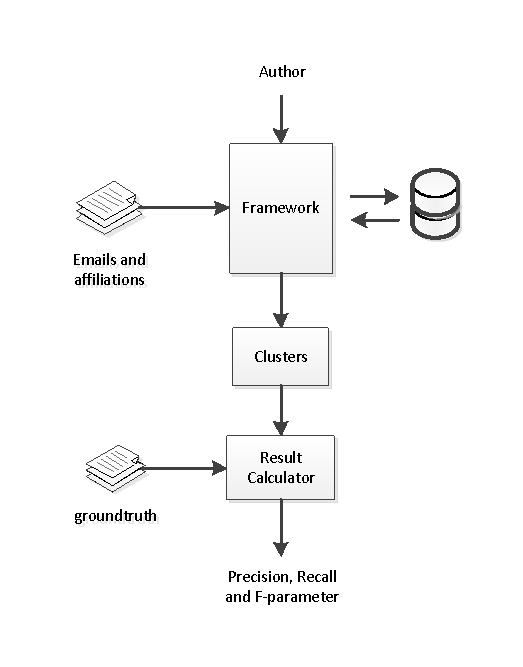
\includegraphics{./fig/testsetup.pdf}
	\label{fig:testsetup}
	\caption{A simplified overview of the test setup starting with the author name and ending with the accuracy results.}
\end{figure}

The result calculator calculates the precision, recall and F measure as defined in \autoref{eq:prf}. Unless explicitly stated otherwise, when we refer to F measure, we mean the $F_{1}$ measure where recall and precision are equally important. These statistical values are calculated for each of the clusters from the ground truth. 

\begin{equation}
	\label{eq:prf}
	\begin{array}{r c l}
		precision & = & \frac{\left|\left\{relevant~documents\right\} \cap \left\{retrieved~documents\right\}\right|}{\left|\left\{retrieved~documents\right\}\right|} \\
		recall & = & \frac{\left|\left\{relevant~documents\right\} \cap \left\{retrieved~documents\right\}\right|}{\left|\left\{relevant~documents\right\}\right|} \\
		F_{\beta} & = & ( 1 + \beta^{2} ) * \frac{precision * recall}{\beta^{2} * precision + recall} \\
	\end{array}
\end{equation}

If we denote the cluster of the ground truth as $C_g$, then the calculated cluster from the graph the result calculator will $C_g$ compare with is given by 

\begin{equation}
	\label{eq:calccluster}
	\min_{\forall c \in calculated~clusters}{\left| C_g \setminus c \right|}
\end{equation}

In \autoref{eq:prf}, we use the terms relevant and retrieved documents. The explanations of these terms are given by the following definitions.

\begin{mydef}
	\textbf{Relevant documents} The publications from the cluster in the ground truth.
\end{mydef}

\begin{mydef}
	\textbf{Retrieved documents} The publications from the cluster calculated by the framework belonging to the cluster in the ground truth, calculated in \autoref{eq:calccluster}.
\end{mydef}

After calculating these statistical values for all the clusters in the ground truth, the mean F measure is calculated to give us an idea of the accuracy for a given test.

\section{Results}

\subsection{Synchronous versus Asynchronous Execution}

Any connection in a pipe network can be configured to be local or asynchronous. Asynchronous connections push the flow in a shared queue of flows that need to be processed. A pool of workers on different machines will poll this queue and resume the flow on their own machines, making the pipe network distributed. We expect this scaling to entail an increase in performance.

We notice that a pipe network that is executed synchronously spends more than 50\% of its time waiting for input. This is because accessing websites, distributed memory or the graph is associated with a certain latency causing pipes to wait for the service to respond. The amount of time spent waiting heavily depends on the characteristics of the input and the hardware. Some inputs require more computation and others more communication. When we run three workers on the same machine, we can already perceive a speedup of 200-300\%.

We expect that distributing the pipes over multiple servers would have a enormous impact on performance. The pipes try to minimize the amount of communication with the graph database as much as possible, making the system more scalable. As we do not have decent server hardware at our disposal, we were not able to test this.

\subsection{Rules}

We have tested the influence of the different rules on the accuracy. For each of the families, we tested the same combination of rules in succession. The F measure for each of these combinations can be seen on \autoref{fig:test-rules}. The combination of all four rules, renders the best result, although sometimes the increase in accuracy from an additional rule is minimal. For "Chen", adding the affiliation rule to the community and email rule even results in a small decrease in accuracy. This is because certain authors are clustered together wrongly. The exact F measures for this combination can be found in \autoref{tab:comparison-dblp}. 

\begin{figure}[htb]
	\centering
		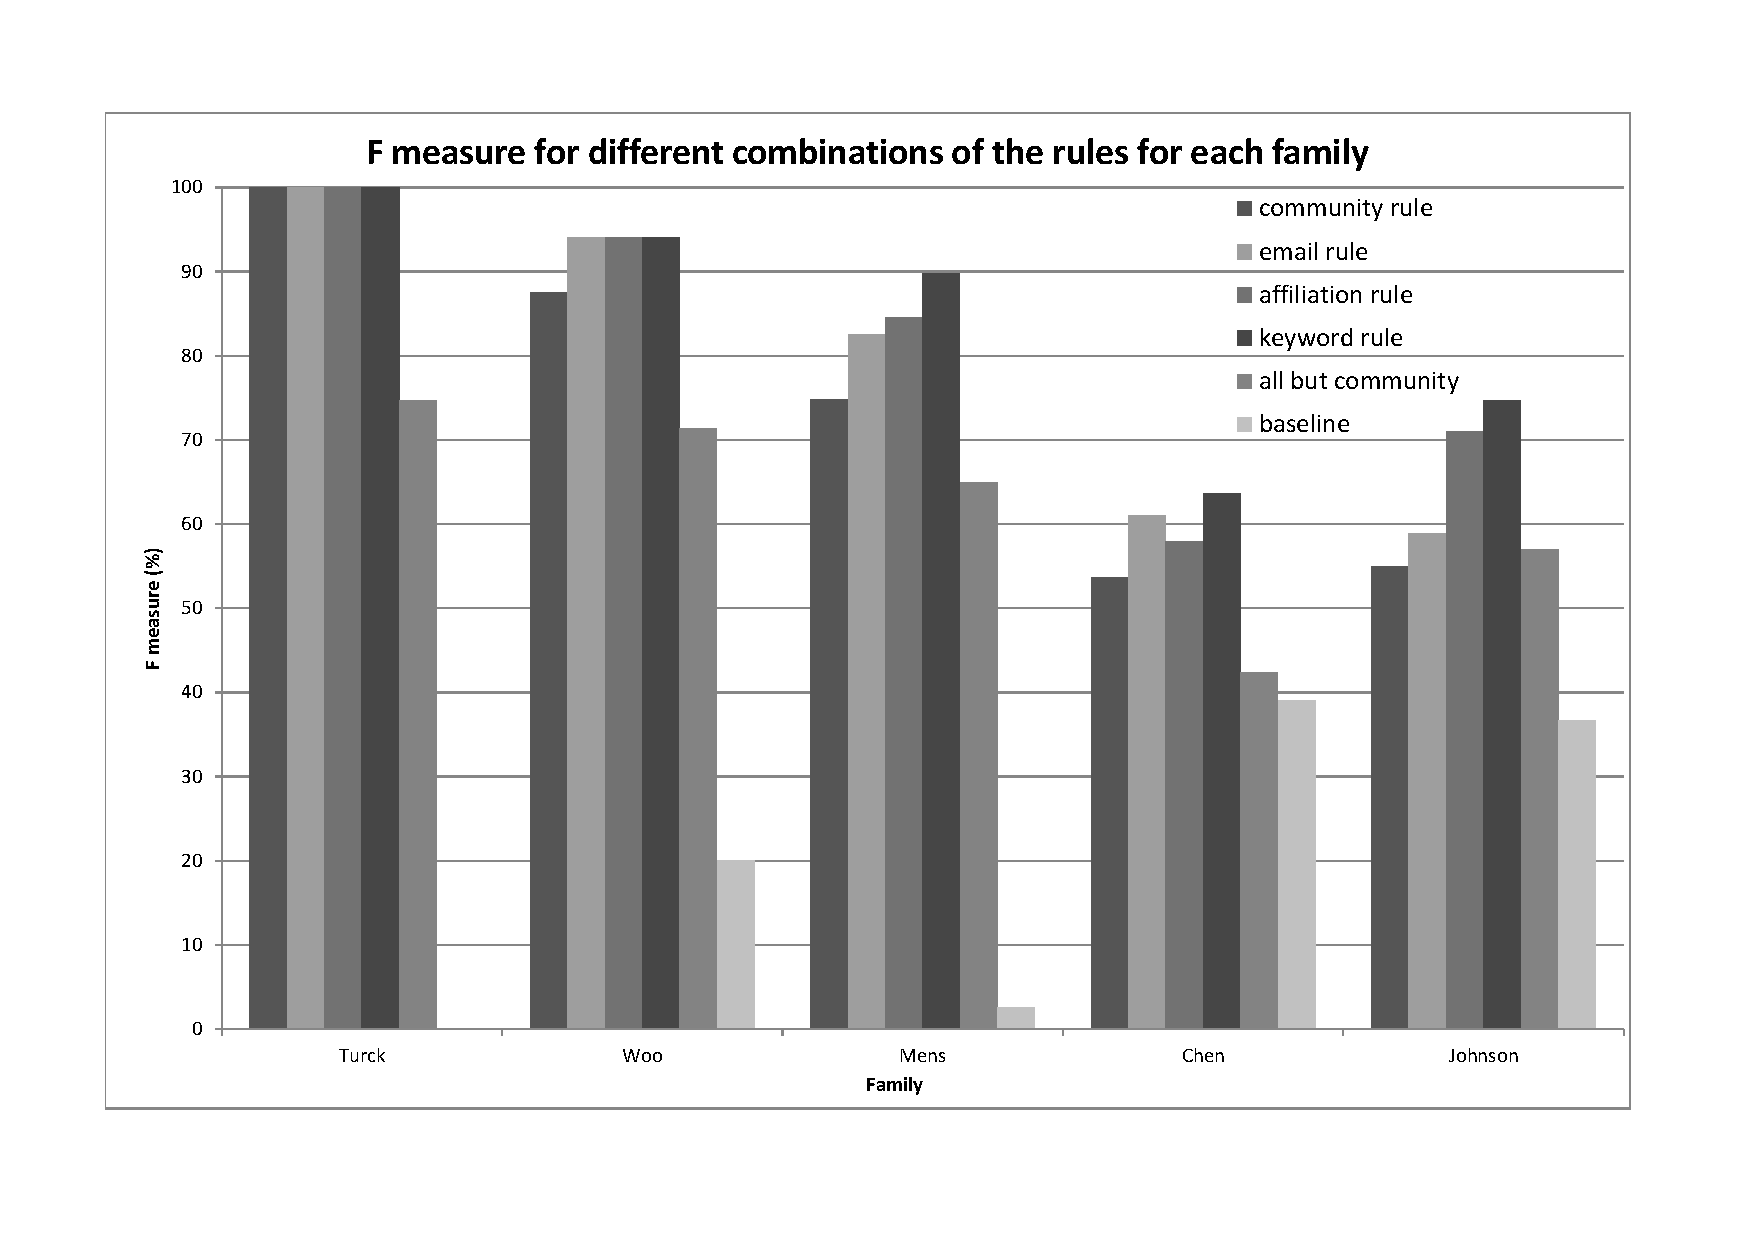
\includegraphics[width=0.80\textwidth]{./fig/test-rules.pdf}
	\caption{A comparison of the accuracy, measured as F score, for the different rules and combinations. The first column shows the use of just the community rule (community rule). The second column shows it in combination with the email rule (email rule). The third rule is a combination of the previous two with the affiliation rule (affiliation rule), while the fourth is a combination of all four rules (keyword rule). The fifth column shows the combination of the email, affilation and keyword rule. The last column gives the so-called baseline, this is the F measure we get when all authors are considered different authors.}
	\label{fig:test-rules}
\end{figure}

The weights we used for the different rules are the same in each of the tests and is the result of \autoref{sub:weights}. We used the weight distribution called "highkey", as denoted in \autoref{table:highkey}, as this distribution yielded the highest average accuracy.


% bespreek figuur

\subsection{Weights}
\label{sub:weights}

We have tested different values for the weights allocated to each of the rules and also the value of $\alpha$ which is used to determine if reclustering should occur. The results are shown on \autoref{fig:test-weights}, while the different distributions are depicted in \autoref{table:distributions}. The average F measure for each distribution over the five families is given by:

\begin{table}[ht]
	\center
	\begin{tabular}{|c|c|}
		\hline
		\bfseries{Distribution} & \bfseries{Average F measure} \\
		\hline
		basic & 81,5\% \\
		\hline
		lowkey & 72,7\% \\
		\hline
		highco & 79,0\% \\
		\hline
		highkey & 84,5\% \\
		\hline
	\end{tabular}
	\caption{The average F measure over the five families for each of the weight distributions.}
	\label{tab:avg-f-distr}
\end{table}

The distribution "highkey" gets the best average accuracy. This distribution gives high values to all properties, favoring a lot of clustering, while the higher alpha makes sure there is still a threshold. Only for family "Johnson", it doesn't get the highest F measure. This can be attributed to too much clustering, resulting in a higher recall, but a lower precision. The actual F measures for this distribution can be seen in \autoref{tab:comparison-dblp}.

\begin{table}[ht]
	\begin{minipage}[b]{0.5\linewidth}\centering
		\begin{tabular}{|c|c|}
			\hline
			\bfseries{Property} & \bfseries{Weight} \\
			\hline
			$\alpha$ & 25 \\
			\hline
			keyword rule & 4\\
			\hline
			community rule & 8\\
			\hline
			affiliation rule & 10\\
			\hline
			email rule & 1000\\
			\hline
		\end{tabular}
		\caption{Basic}
	\end{minipage}
	\begin{minipage}[b]{0.5\linewidth}
		\centering
		\begin{tabular}{|c|c|}
			\hline
			\bfseries{Property} & \bfseries{Weight} \\
			\hline
			$\alpha$ & 25 \\
			\hline
			keyword rule & 1\\
			\hline
			community rule & 8\\
			\hline
			affiliation rule & 10\\
			\hline
			email rule & 1000\\
			\hline
		\end{tabular}
		\caption{Lowkey}
	\end{minipage}
	\begin{minipage}[b]{0.5\linewidth}\centering
		\begin{tabular}{|c|c|}
			\hline
			\bfseries{Property} & \bfseries{Weight} \\
			\hline
			$\alpha$ & 25 \\
			\hline
			keyword rule & 1\\
			\hline
			community rule & 50\\
			\hline
			affiliation rule & 10\\
			\hline
			email rule & 1000\\
			\hline
		\end{tabular}
		\caption{Highco}
	\end{minipage}
	\begin{minipage}[b]{0.5\linewidth}
		\centering
		\begin{tabular}{|c|c|}
			\hline
			\bfseries{Property} & \bfseries{Weight} \\
			\hline
			$\alpha$ & 25 \\
			\hline
			keyword rule & 10\\
			\hline
			community rule & 50\\
			\hline
			affiliation rule & 10\\
			\hline
			email rule & 1000\\
			\hline
		\end{tabular}
		\caption{Highkey}
		\label{table:highkey}
	\end{minipage}
	\caption{Weight distributions with the name of each distribution as used in \autoref{fig:test-weights}}
	\label{table:distributions}
\end{table}

\begin{figure}[htb]
	\centering
		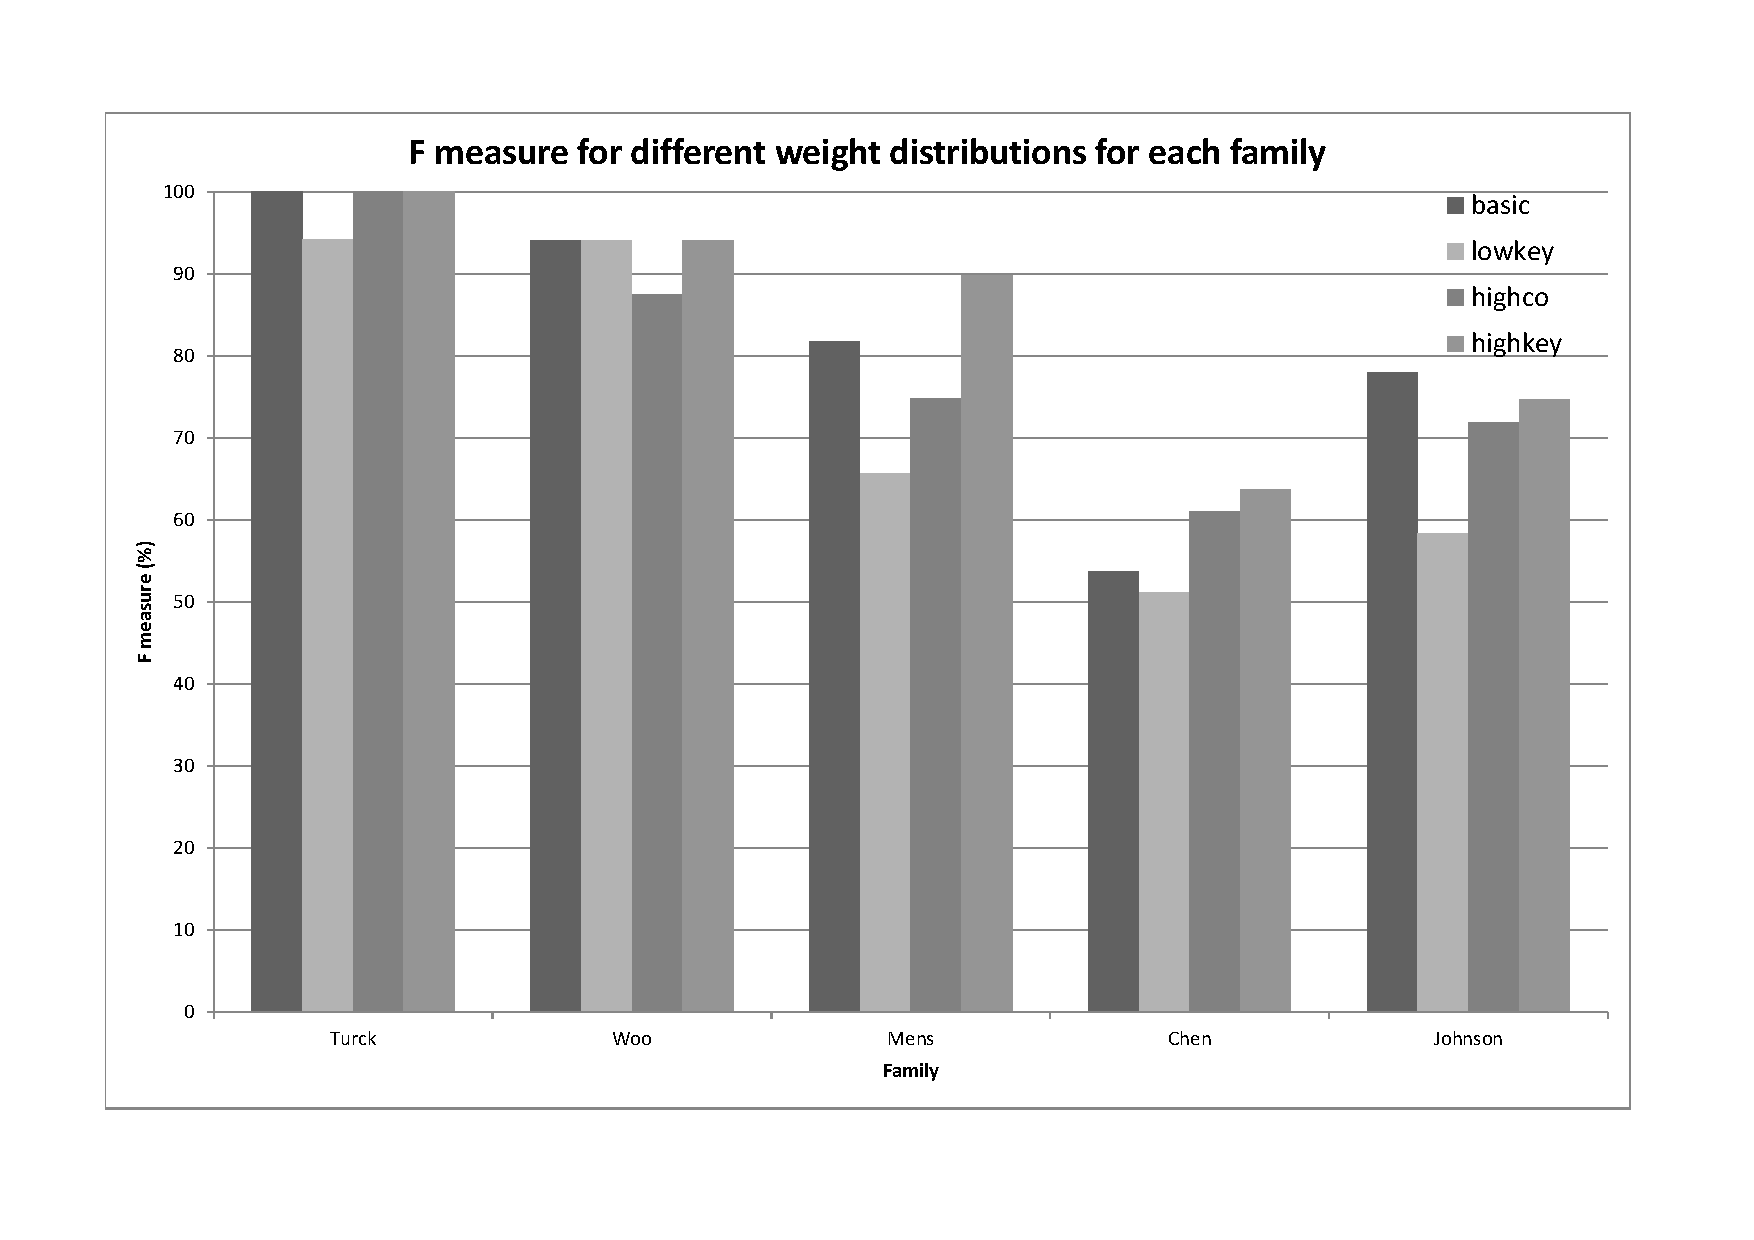
\includegraphics[width=0.80\textwidth]{./fig/test-weights.pdf}
	\caption{The F measure for different weight distributions for each family. The weight distributions, from left to right, are "basic", "lowkey", "highco" and "highkey". The actual value for the distributions is shown on \autoref{tab:avg-f-distr}.}
	\label{fig:test-weights}
\end{figure}

\subsection{Comparing to DBLP}

We have calculated the F measure for each of the families as they are divided on DBLP, to make a comparison with our own results. The values are shown on \autoref{tab:comparison-dblp}. The divisions for "Turck" and "Mens" are completely correct, the other three are far less accurate with "Chen" having an astonishingly low F measure of $2.73\%$. We compare the F measure to our highest average scoring distribution, "highkey". We also compare the mean F measures and a weighted variation of the mean measure which is calculated using the following formula ($F_X(f)$ is the F measure for family name $f$ for $X$):

	\[
	\sum_{f \in families}{\frac{F_{X}(f)}{|f_{publications}} * N},~X \in \left\{DBLP,highkey\right\},~N = total~number~of~publications
\]

Our framework scores $14\%$ to $17\%$ better than DBLP, depending on how the mean value is measured.

\begin{table}
	\centering
		\begin{tabular}{|c|c|c|c|c|c|c|c|}
			\hline
			& \bfseries{Turck} & \bfseries{Woo} & \bfseries{Mens} & \bfseries{Chen} & \bfseries{Johnson} & \bfseries{Mean} & \bfseries{Weighted} \\
			\hline
			\bfseries{DBLP} & 100.0\% & 87.5\% & 100.0\% & 2.7\% & 62.8\% & 70.6\% & 61.8\% \\
			\hline
			\bfseries{Highkey} & 100.0\% & 94,1\% & 89,8\% & 63,7\% & 74,7\% & 84,5\% & 79,0\% \\
			\hline
		\end{tabular}
	\caption{Comparison of the F measures for the different families as they are divided on DBLP and as calculated by our framework. The last columns give the mean F measure and a weighted distribution based on the number of papers in each family.}
	\label{tab:comparison-dblp}
\end{table}

%\include{gerelateerdwerk}
%\include{gelijkheid}
%\include{aanbevelingen}

\chapter{Conclusion and Future Work}

%Our system only provides a snapshot of the expertise on a given time, it should be better if we could provide an overview in time.

\section{Conclusion}

In this master's thesis we examined the opportunities using the semantic web and data processing. We found out that the possibilities within expert finding and author disambiguation are challenging and can contribute in solving a real-life problem. At the end of this informative investigation, the objective became clear: creating a framework that is able to disambiguate authors and allows users to find experts for a certain subject, while keeping it extensible for future additions.

% Wat is juist zo naief aan de eerste aanpak en waarop is deze precies gebaseerd, in 1 zin

We started with a naive approach for the framework. We focused on what we knew and were comfortable with rather than the problem we had to solve. It lacked both in performance and scalability, while the usage of a relational database would render it unrealizable. Profound inspection of this first version of the framework, however, learned us that in order to create a good one, it would have to amplify the following five foundations:

\begin{enumerate}
	\item All instances are considered different authors until proven otherwise.
	\item No decision is made permanent.
	\item Any information is considered partial information.
	\item A constantly changing input asks for a constantly changing output.
	\item The stream of informaton is endless.
\end{enumerate}

% Iets over graaf en regels

With these foundations in mind, we first created a theoretical model. This model consists of three layers that integrate structural, informational and algorithmic aspects. It deals with the main difficulties of author disambiguation, while minimizing the problem domain. We also explain how to process the (partial) information in order for similarities to be found. 

Rules drive the entire flow in our framework by converting novel facts into similarities that group instances with authors through clustering. The four rules we defined for our framework are:

\begin{enumerate}
	\item \textit{Community Rule} Exploiting the fact that authors often work together with the same co-author.
	\item \textit{Interest Rule} The subjects of publications of the same author are usually located within the same field of research.
	\item \textit{Email Rule} Authors with the same email address, are most likely the same person.
	\item \textit{Affiliation Rule} Authors are more likely to work at one affiliation at a given time.
\end{enumerate}

We implemented this theoretical model with pipes and filters using Ruby, Java, key-value store Redis, Resque for scaling and the Tinkerpop stack for the graph representation. The usage of pipes and filters allows for modifiability. New pipes can easily be plugged into the flow which enables the convenient addition of extra information sources or new rules while the performance and scalability remain intact.

Clustering is the process that is responsible for grouping of authors based on the calculated similarities, a key component of our framework. We implemented the dynamic clustering algorithm proposed in \cite{saha2006dynamic} which is based on minimum-cut trees. The quality of the clusters is guaranteed to be the same as its static counterpart, while it is a lot faster as it considers much smaller subgraphs. We added an extra case to the proposed algorithm, exploiting the fact that our framework often has a succession of small similarities connecting the same clusters. This extra case permits the most resource-intensive case to be postponed and executed less frequently.

Finding experts using a set of keywords is easily attainable within our framework, though we do not provide a user-friendly interface for inspecting these experts. However, the graph can be directly queried for these keywords and the corresponding authors, ordered by decreasing relevance, can be obtained with a simple traversal.

We tested the framework thoroughly using a manually annotated testset of just over 1000 publications. We showed the impact of each of the rules on the accuracy, clarifying that the combination of all four of them render the best average results, although the increased accuracy from the addition of a rule is minimal in certain cases. We also examined the accuracy using different distributions for the rules and we noticed that the community rule had the biggest impact. Finally, we also compared the accuracy of our framework with the accuracy of DBLP for the tested authors and concluded that our framework transcends DBLP by $14\%$ or $17\%$, depending on how the mean accuracy is calculated.

\section{Future Work}

There are many possible additions to be made to the framework. Adding extra online sources by writing new pipes can help us in the search for more information about each author and give us a better view for disambiguation. Additional, extra rules could be written to translate the newly acquired information to similarities between authors which were previously unknown.

Another improvement is enabling the usage of negative weights for similarities. This could undo previously calculated results, when there is reason to believe two instances are not connected. Related to the addition of using negative weights, would be the possibility to have immutable decisions. Especially if this decision is that two authors can never be the same. A simple reason that comes to mind is that they are both co-authors of the same publication.

Using an actual category tree containing a large overview of categories, could help in calculating more accurate similarities between keywords that are not the same, but are bound to the same area of expertise. This could also enable giving higher weights to keywords that are more specific for a certain subject.

Another addition would be using the abstract or even the actual text of the publication for deciding the category. This could get far better results are publication titles are sometimes vague and open for interpretation. Getting the abstract could be achieved by writing plugins for the most popular digital libriries by using web scraping.

% Rekening houden met negatieve gewichten
% Absolute vaststellingen kunnen maken : deze 2 auteurs zijn ZEKER verschillend en moeten altijd zo blijven
% Opstellen van categorie boom om betere keyword results te krijgen
% Grotere gewichten toekennen voor woorden die meer subject specifiek zijn
% Scalability fixen :o
% Meer bronnen opnemen
% Category bepaling niet enkel op basis van titel, maar ook abstract of zelfs volledige tekst => plugins schrijven voor verschillende paper aanbied sites (zijn er slechts een paar)
% 

% appendices
%\appendix

% hier worden de appendices ingevoegd (\includes)


%\include{referenties}

% De bibliografie en de index
\bibliography{collection}
\backmatter

% eventueel: lijst van figuren en tabellen
\listoffigures
\listoftables

% lege pagina (!!)

% kaft

\end{document}
